\chapter[Electrons][Electrons]{Electrons}
\label{chapter:electron} 

High energy electron signatures are important elements of searches and measurements at hadron colliders, because they signal the presence of important electro-weak processes in the event. Requiring well-identified electrons in collision events suppresses the overwhelming rate of strong-force mediated scattering and allows for the collection of a manageably-sized dataset with interesting physics for study. For this reason, electron signatures form one of the two pillars of the HLT trigger at ATLAS, as discussed in Chapter~\ref{chapter:lhc}, and rigorous electron identification is an important piece of many ATLAS analyses. This section summarizes the development of ATLAS electron identification for the high luminosity 2011 and 2012 datasets and discusses the techniques involved in measuring the electron identification efficiency. 

\section{Identification of Electrons at ATLAS}

%pictures and example figures

Electron reconstruction is discussed briefly in Chapter~\ref{chapter:lhc} and, in depth here~\cite{ATLAS-CONF-2014-032}. The result of electron reconstruction is called an electron candidate, which is comprised of a narrow calorimeter energy cluster with $|\eta| < 2.47$ and and ID track that matches loosely in $\eta$ and $\phi$. If the electron has $|\eta| < 2.01$, the ID detector track is fiducial to the TRT and has the possibility of having high-threshold hits, indicative of transition radiation (TR). Electron cluster reconstruction is extremely efficient. The track-matching requirement is less efficient, because the presence of hard bremsstrahlung may in certain cases cause the electron cluster and emitted photon cluster to have a wide separation in the calorimeter \cite{ATLAS-CONF-2012-047}. Figure \ref{figure:electron_reco} shows the reconstruction efficiency as a function $|\eta|$ for an example \pt\ bin as well as a plot of the amount of material in front of the EM calorimeter. The efficiency loss at high $|\eta|$ is caused mostly by material-induced hard bremsstrahlung.  

\begin{figure}[!t]
\centering 
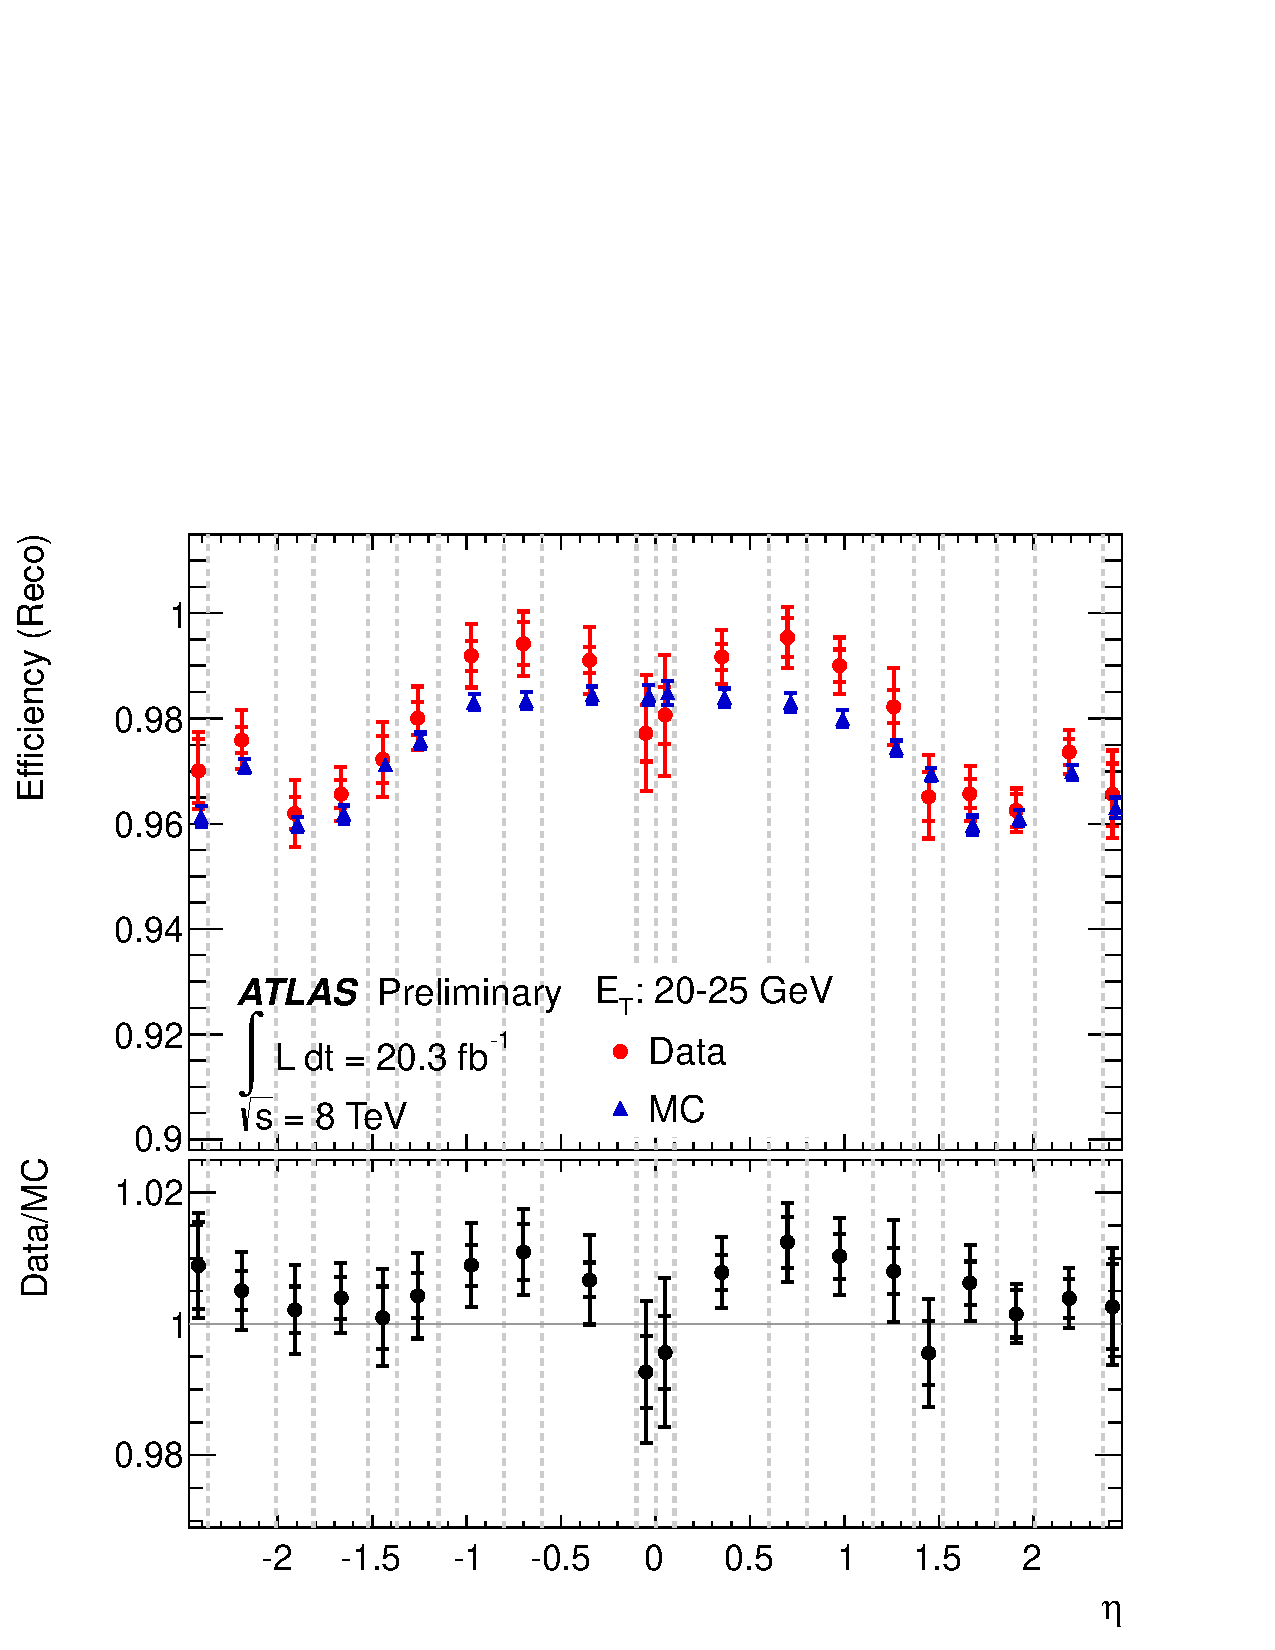
\includegraphics[width=0.40\textwidth]{figs/electron/fig_26b}
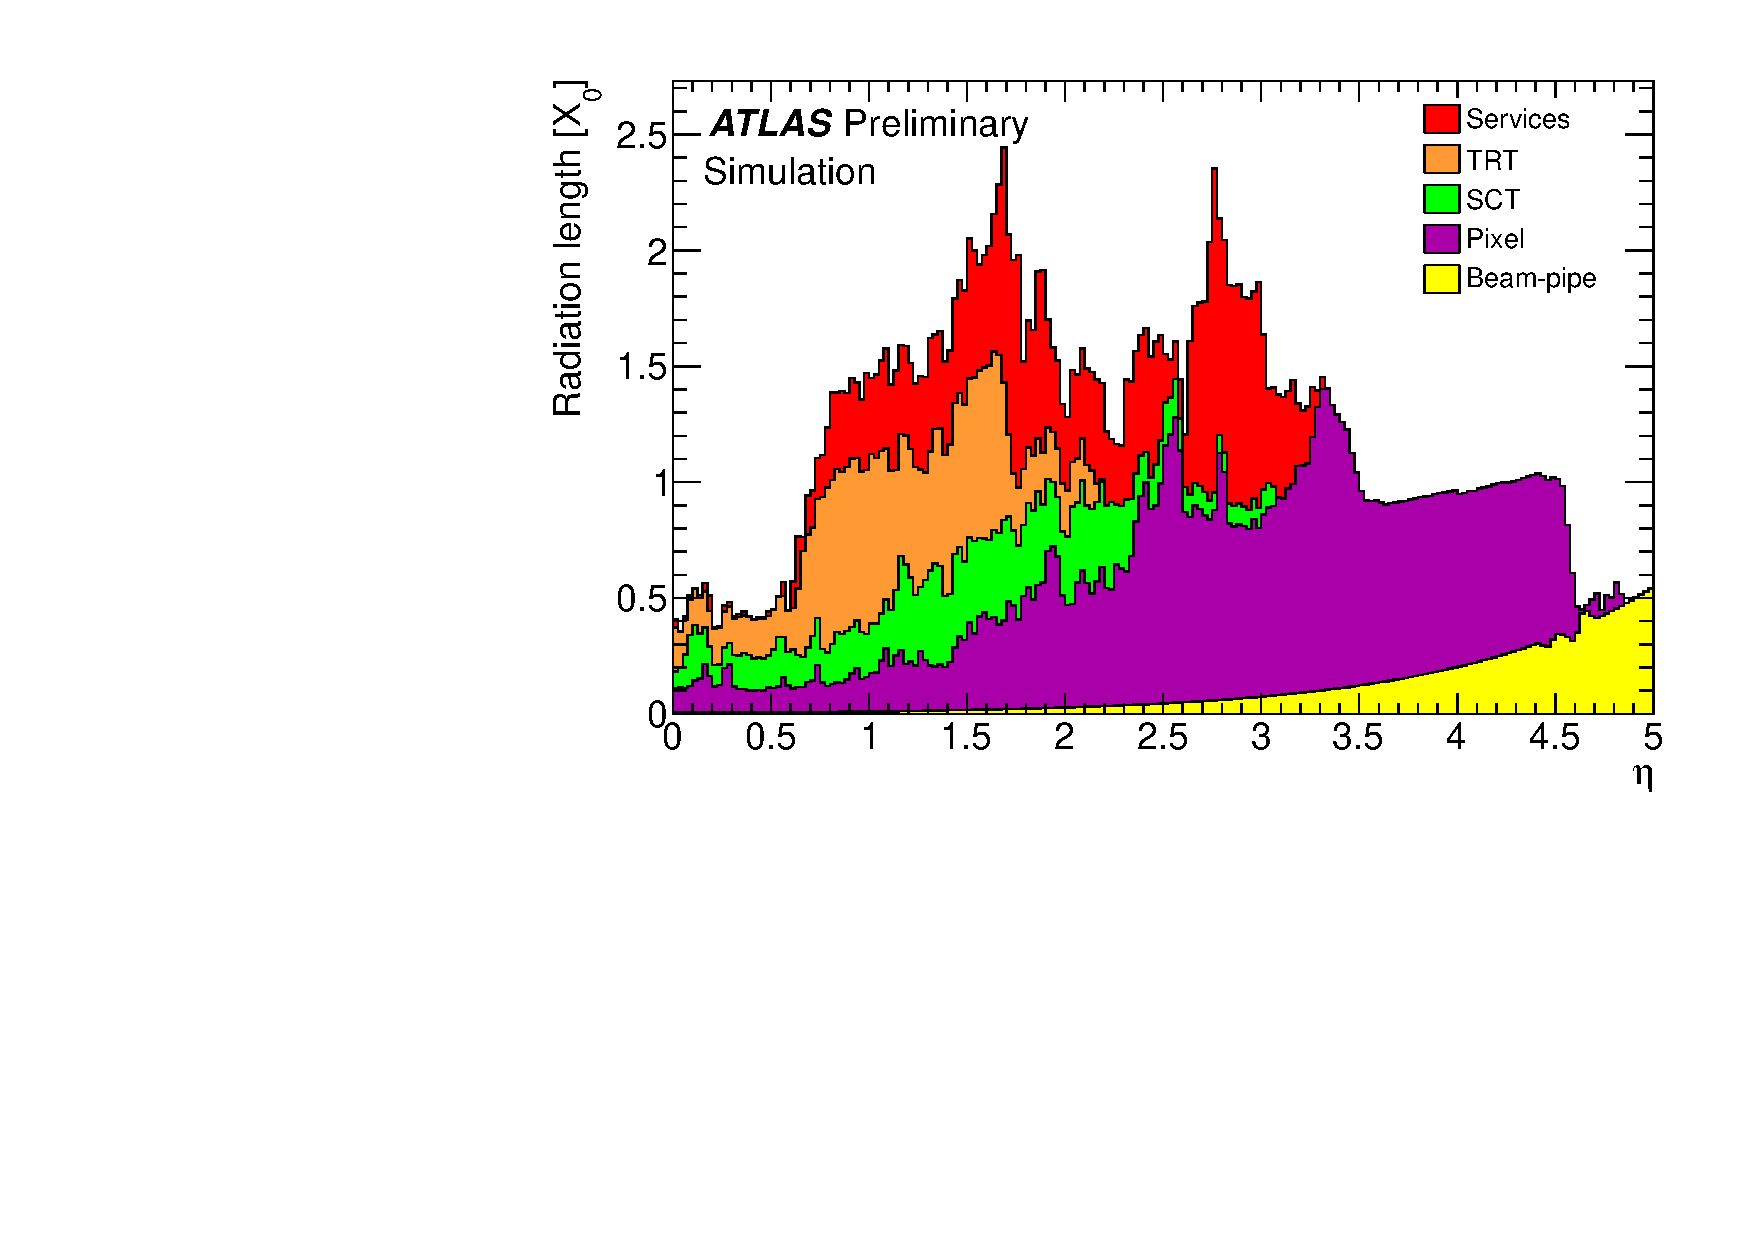
\includegraphics[width=0.40\textwidth]{figs/electron/fig_01b}
\caption{Electron reconstruction efficiency for an example \pt\ bin versus $|\eta|$. The drop in efficiency at higher values of $|\eta|$ is directly attributable to the increase in the amount of material in front of the EM calorimeter (left). The material causes bremsstrahlung, which makes track-cluster matching more difficult for electrons}
\label{figure:electron_reco}
\end{figure}



Objects that are not isolated electrons are often reconstructed as electrons, as the reconstruction requirements are quite loose. Objects that often `fake' isolated electrons are light quark and gluon jets, heavy flavor jets that include real decays to electrons, and converted photons. Light quark and gluon jets fragment into a number of collimated hadronic particles. In rare cases, the jet may fragment most of its energy into a single charged pion, which showers early in the EM calorimeter and fakes an electron signature. In other cases, the jet may fragment mostly into a neutral pion, which subsequently decays into a pair of photons. If one of these photons converts, a track will point to the EM energy cluster and possibly fake an electron signature. These cases would result in a reconstructed electron candidate. Although the probability for these misidentifications to happen is small, the enormous jet production rate means that it is a significant background. In general, light quark and gluon jet `fakes' have larger transverse shower profiles and more energy leakage into the hadronic calorimeter. For the neutral pion case, there are generally two separated showers for lower energy decays. For both cases, there are often other particle signatures nearby.  
Heavy-flavor jet decays and photon conversions contain real electrons. However, heavy flavor decays also involve the production of additional hadronic particles within the jet. Both photon conversion and heavy flavor decays involved secondary vertices displaced from the primary interaction point. 


\begin{figure}[!t]
\centering 
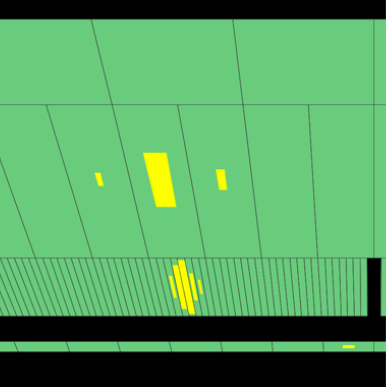
\includegraphics[width=0.33\textwidth]{figs/electron/photon.png}
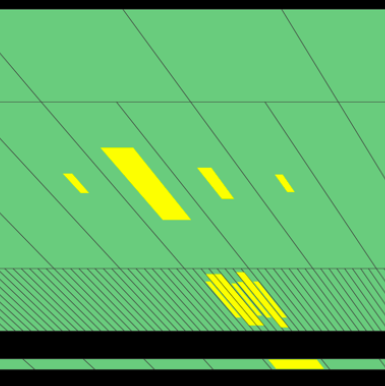
\includegraphics[width=0.33\textwidth]{figs/electron/pi0.png}
\caption {Example single photon (left) and $\pi^0\rightarrow\gamma\gamma$ (right) signatures in the ATLAS EM calorimeter. The fine segmentation of the cells in the strips allows for the distinguishing of two nearby showers from one shower
and is used in electron identification}.
\label{figure:electron_pi0}
\end{figure}

In order to distinguish these fake signatures from real, isolated electrons, electron identification algorithms use a number of reconstructed variables describing the electron shower in the detector and the electron track. The details of the calculated variables can be found here~\cite{ATL-PHYS-PUB-2011-006}. In general, electron identification takes advantage of the narrowness of isolated electron shower in the transverse plane and lack of energy deposition in the hadronic calorimeter. The transverse variables include measurements of the shower width in both layer 2 and the strips, where more refined measurements are possible. In fact, the strips were designed to separate single photon and electron showers from multiple showers from neutral pion decays, shown in Figure \ref{figure:electron_pi0}. The shower width variables are generally measured mostly in $\eta$ as bremsstrahlung tends to smear the electron energy in $\phi$. Electron tracks are required to have an adequate number of hits in the Pixel Detector, SCT and TRT. These hit requirements, especially the b-layer requirement suppress electron conversions which occur in the detector material. Track-cluster matching and geometric impact parameter variables require ID tracks to match the calorimeter energy well and to arise from the primary interaction point. Electrons with tracks explicitly associated with a conversion vertex can be rejected. Finally, the high threshold fraction of hits on the track, made by transition radiation, is an uncorrelated discriminator of pion and electron tracks. Figure~\ref{figure:electron_tr} shows the average high threshold hit probability for pions and electrons as a function of their \pt. 

\begin{figure}[!t]
\centering 
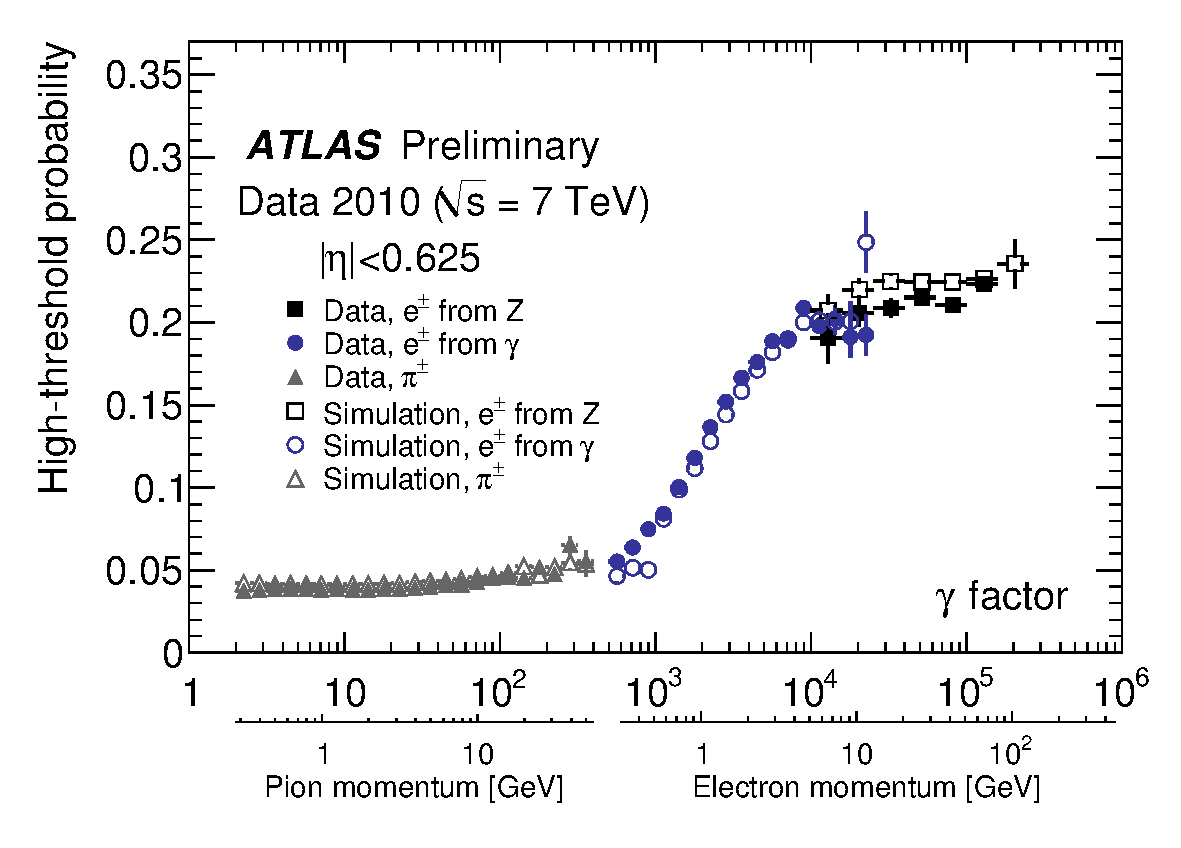
\includegraphics[width=0.69\textwidth]{figs/electron/TRFractionBarrel-eps-converted-to}
\caption{Electron and pion track high threshold probabilities as a function of their transverse momenta. The two scales are united through the $\gamma$-factor, on which the TR probability depends directly. Electron tracks are much more likely to have high threshold hits at electron energies typical of electro-weak decays.}  
\label{figure:electron_tr}
\end{figure}


Electron identification algorithms make selections in 9 bins of $|\eta|$, [0.10, 0.60, 0.80, 1.10. 1.37, 1.52, 1.81, 2.01, 2.37, 2.47] and bins of \pt, [7, 10, 15, 20, 30, 40, 50, 60, 70, 80$+$] GeV. The $|\eta|$ binning changes with the calorimeter geometry, which in turn affect the shower shape distributions. The shape of most of the identification variable distributions, tracking and calorimeter, are \pt\ dependent.  



\subsection{2011 Menu}

Electron identification in 2011 was accomplished through rectangular cuts on the identification variables at 3 operating points: Loose, Medium and Tight. The medium operating point was used online as the primary electron trigger. At the beginning of the 2011 run, the 3 operating points possessed the same cut-values, but tighter operating points had cuts on more variables. The Loose operating point only cut on shower shape variables in layer 2 and hadronic leakage, the medium operating point added cuts on shower width variables in the strips, and tight added TR cuts, strict-track cluster matching, conversion rejection and a b-layer requirement. This menu, called the `IsEM' menu, was the first fully data-optimized cut menu for electrons. 

The demands of increasing luminosity demanded a tightening of the medium operating point midway through the data-taking, in order to maintain a EF trigger rate of around 20-25 Hz on the primary electron trigger. To accomplish this, variables cut on at the tight operating point were added to the medium operating point, and the entire set of cuts was optimized to provide the targeted fake rejection and reduction in the trigger rates at the highest possible efficiency. The same procedure was applied to the loose operating point, where the target was to provide an efficiency of 95\% and the highest possible fake rejection. The re-inventing of the menu in this way allowed for not only better performance, due to the inclusion of more variables, but a more stable tightening of the backgrounds from loose to medium to tight, where the same background types were targeted at each level. The new menu was called the `IsEM$++$' menu and the operating points were renamed `Loose$++$', `Medium$++$' and `Tight$++$'. Figure~\ref{figure:electron_isemvpp} shows the comparison of the operating points for the new menu and old menu.

\begin{figure}[!t]
\centering 
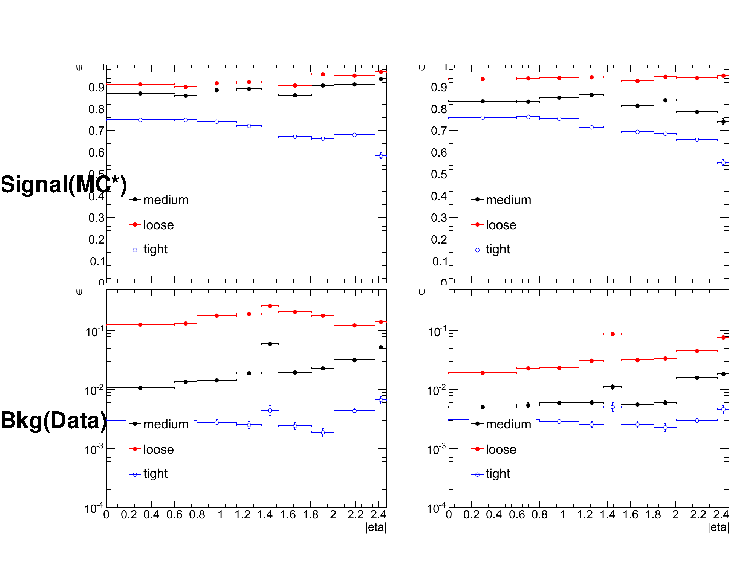
\includegraphics[width=0.80\textwidth]{figs/electron/isEMvsisEMPP.pdf}
\caption {Comparison of the `IsEM' (left) and `IsEM$++$' electron identification operating points for Loose, Medium, and Tight. The efficiency as a function of $\eta$ for an example \pt\ bin is shown on top and the background rejection is shown on the bottom}.
\label{figure:electron_isemvpp}
\end{figure}

\subsection{2012 Menu and Pile-up}

Improvements in the running conditions for 2012, in particular narrowing the transverse beam emittance and size, resulted in large increase in number of proton-proton interactions during every 50 ns bunch crossing. In 2011 the average number of reconstructed primary vertices in each event, an indicator of the number of interaction per bunch crossing, was around 7, while in 2012 the average grew to 25. Some events during 2012 running had 40 reconstructed primary vertices.

The increase in energy in the calorimeters from these additional collisions, called pile-up, caused a worsening of the resolution of electron identification variables, particularly the shower shapes and hadronic leakage. The presumed cause was the increase in the number of showers of low energy hadronic particles near electrons.  Figure~\ref{figure:electron_pu} shows two example distributions, the hadronic leakage (R$_{Had}$) and the transverse shower profile (R$_{\eta}$), for high and low pile-up conditions. The distributions shows a clear widening for higher pile-up which results in a loss of efficiency. 

\begin{figure}[!t]
\centering 
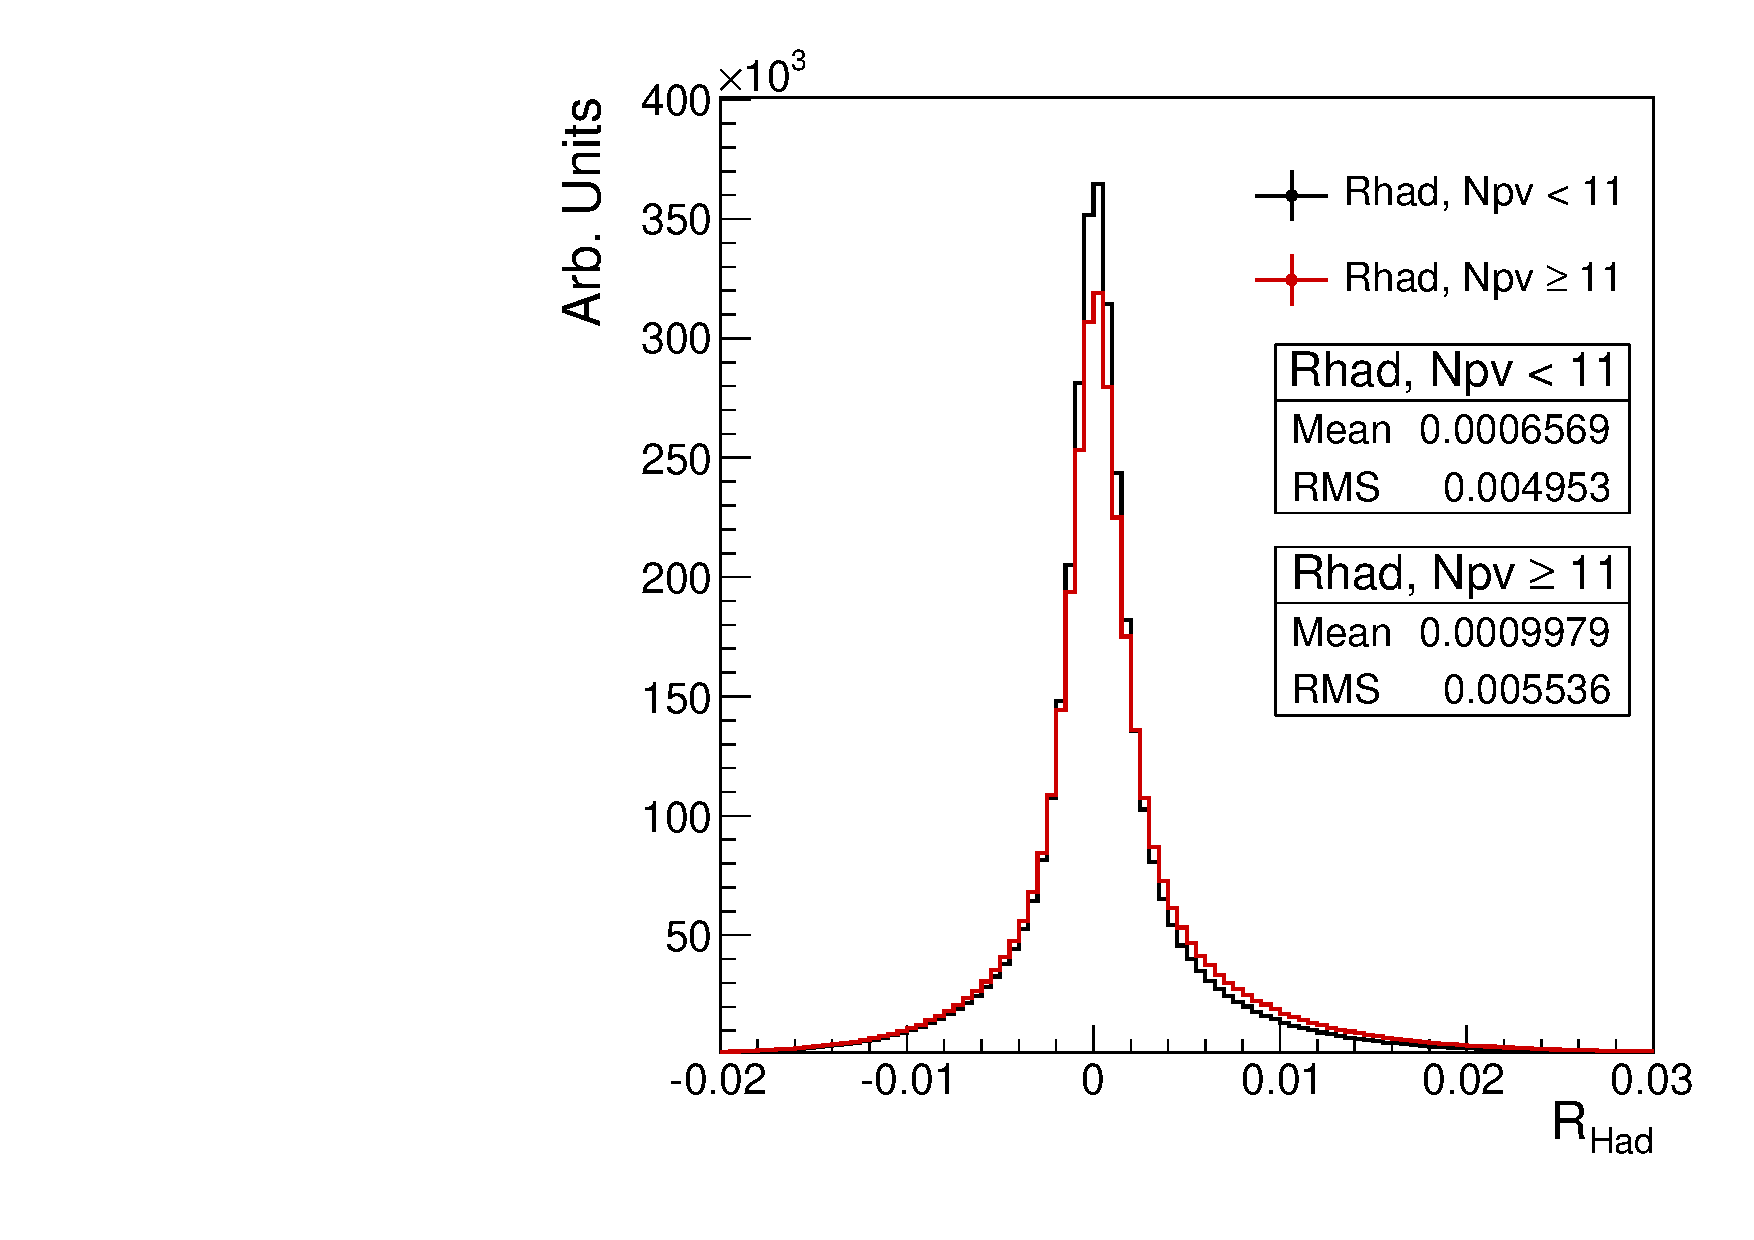
\includegraphics[width=0.40\textwidth]{figs/electron/rhad_npv}
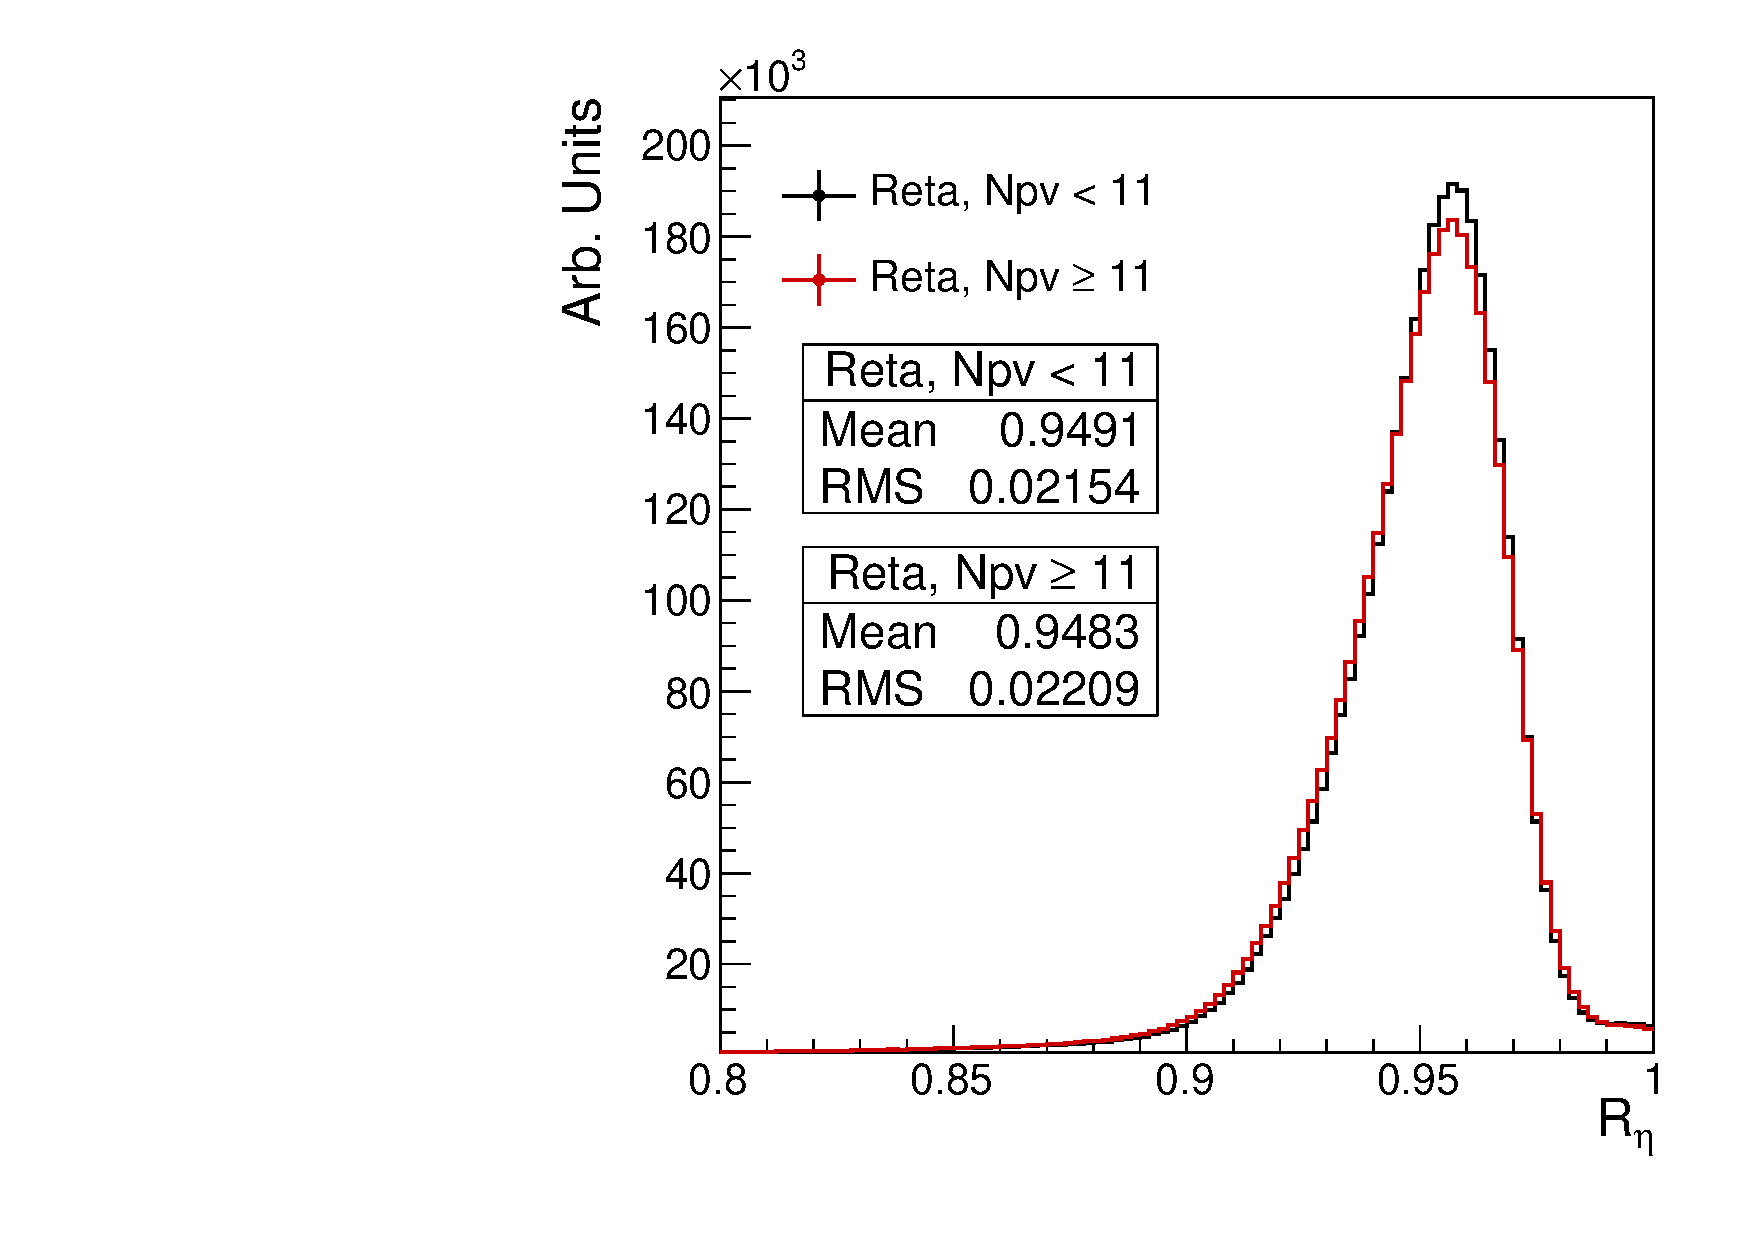
\includegraphics[width=0.40\textwidth]{figs/electron/reta_npv}
\caption {Electron hadronic leakage fraction (R$_{Had}$) and transverse shower profile (R$_{\eta}$) in layer 2 for high and low pile-up conditions. Pile-up is measured here as the number of primary vertices in the event.}
\label{figure:electron_pu}
\end{figure}


In order to combat this loss, the `IsEM$++$' menu was once again optimized to have a flatter efficiency profile as a function of the amount of pile-up in the event with similar performance to the 2011 menu. The strategy for this menu was to loosen selections on variables sensitive to pile-up energy. It was expected and confirmed that relying more on the strip variables for the shower shape selection and the energy in layer 3 of the EM calorimeter for the hadronic leakag would sample a smaller volume of the calorimeter and thus be less sensitive to additional energy in the neighborhood of the electron. The strategy is outlined pictorially in Figure~\ref{figure:electron_schematic}.  

\begin{figure}[!t]
\centering 
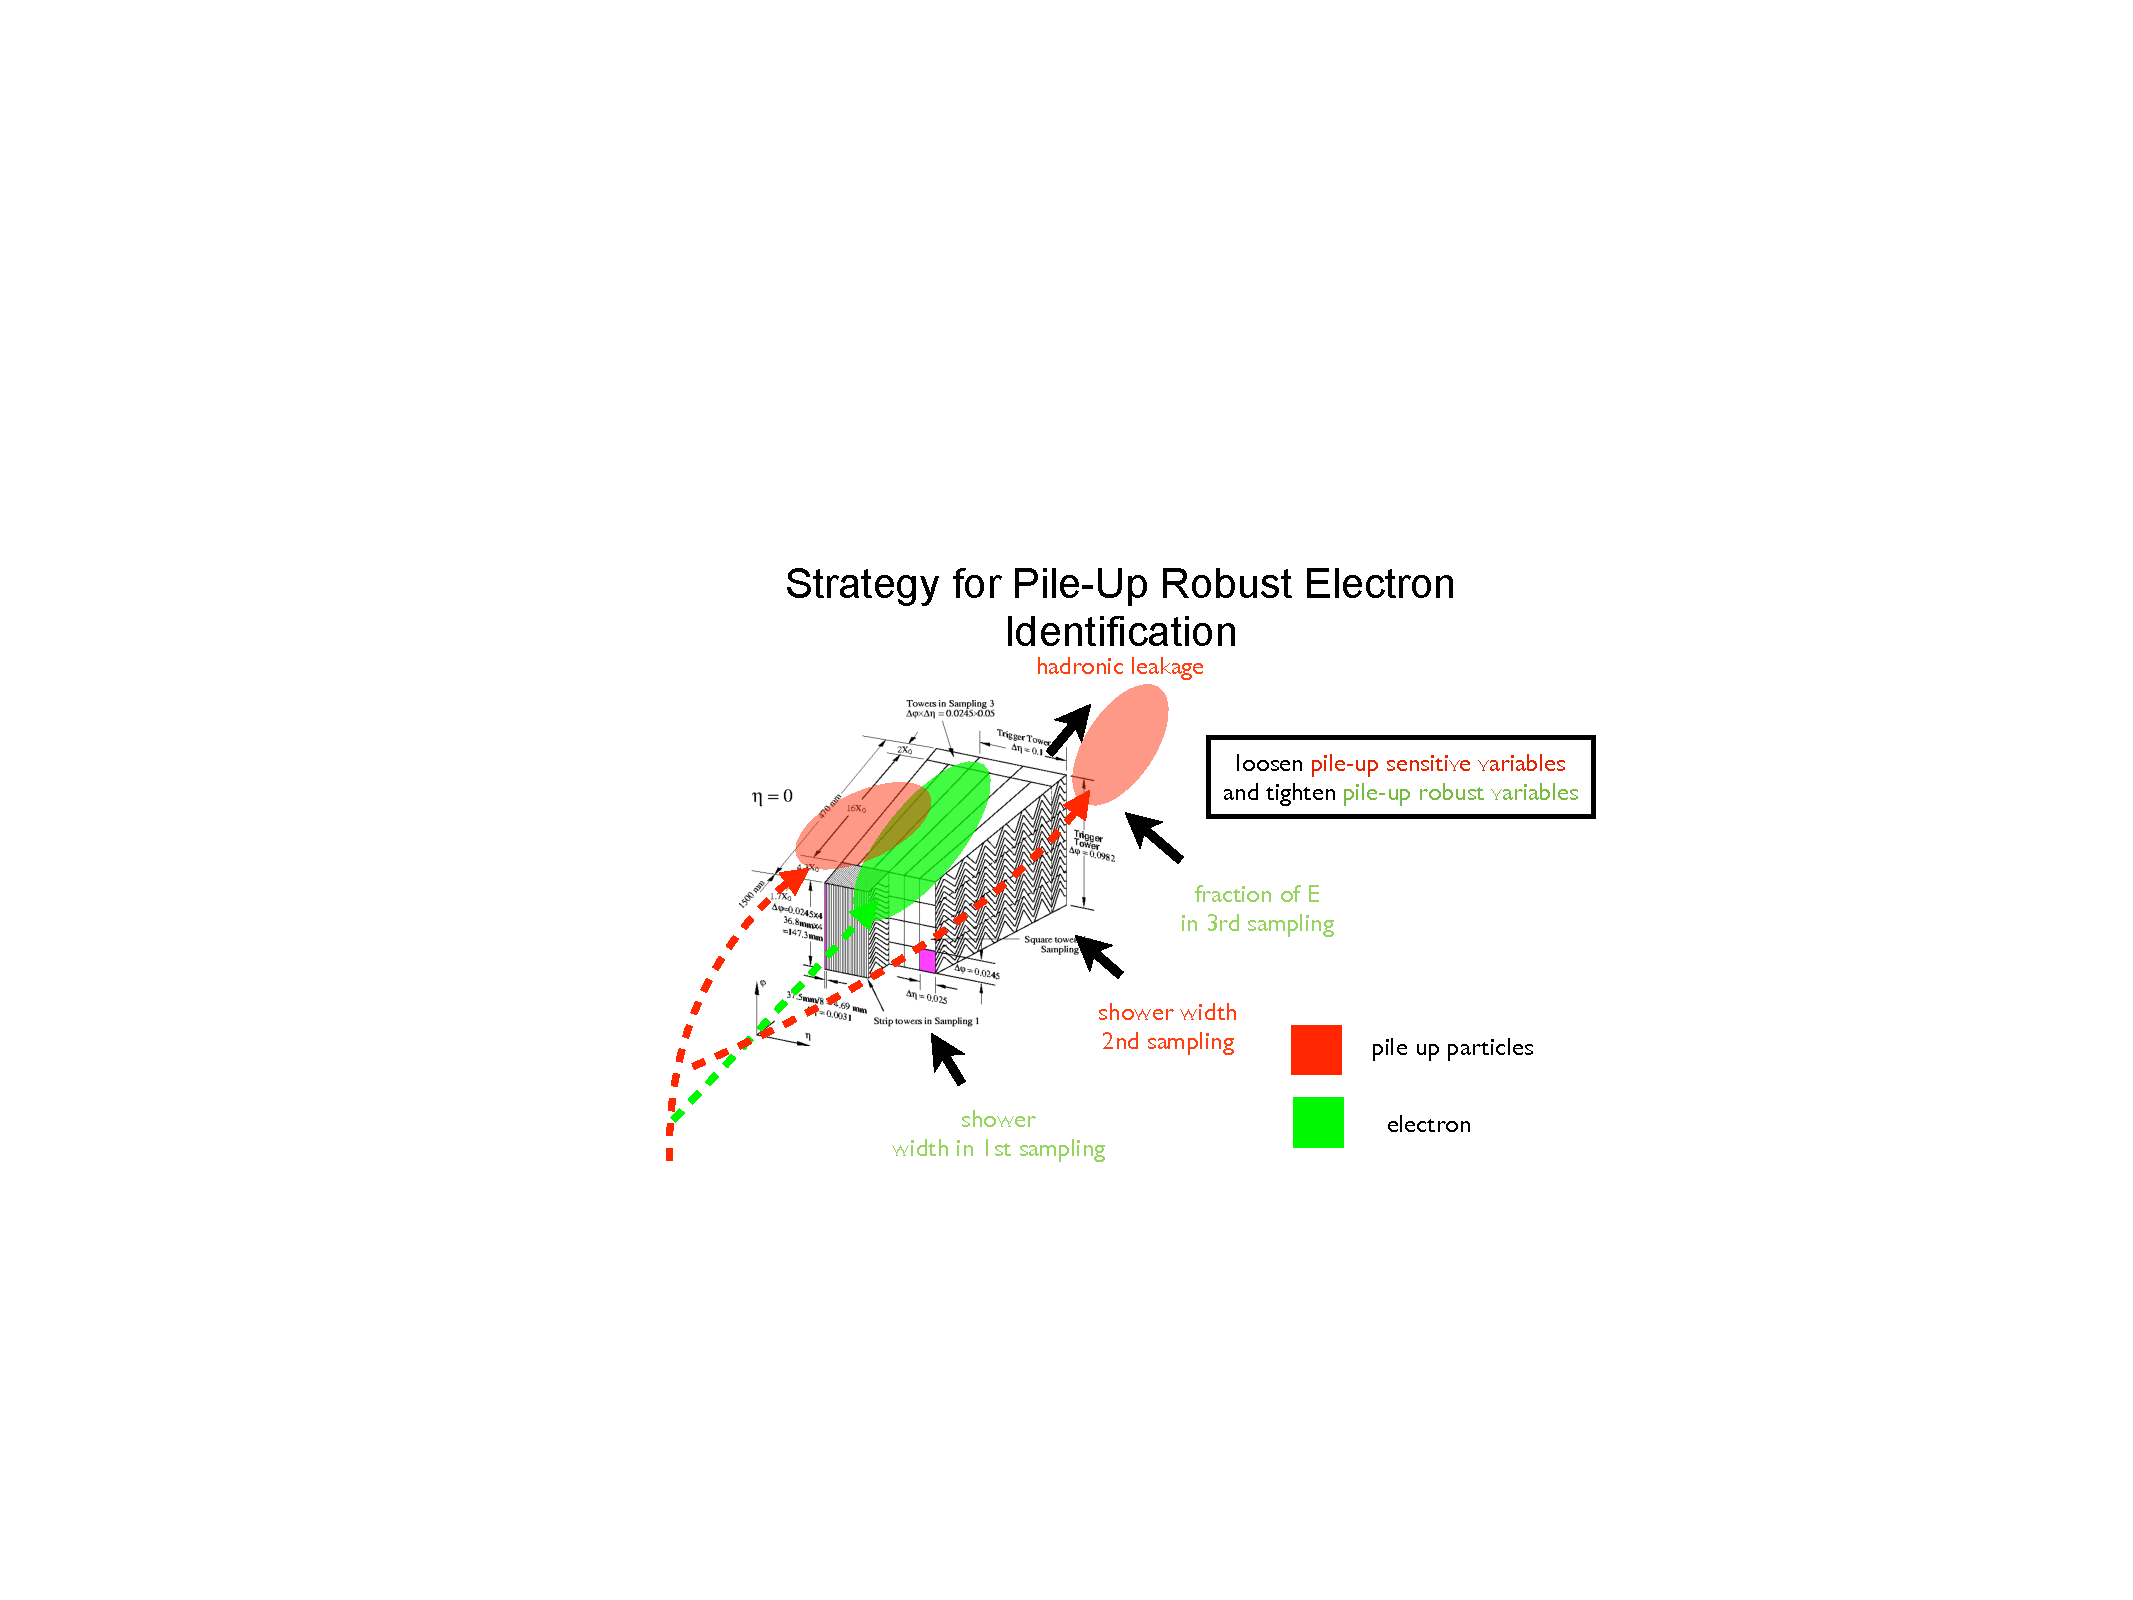
\includegraphics[width=0.69\textwidth]{figs/electron/schematic_pileup}
\caption{Schematic of the strategy to reduce the pile-up dependence of electron identification. A EM calorimeter wedge is shown overlaid with example electron (green) and pile-up particle (red) signatures. The strategy is to loosen the dependence of the identification on layer 2 and the hadronic calorimeter, which sample large volumes, and tighten selection on variables in the the 3rd layer and strips, which sample smaller volumes.} 
\label{figure:electron_schematic}
\end{figure}


The efficiency of the 2011 operating points compared to the 2012 operating points is shown in Figure~\ref{figure:electron_2012_2011}, demonstrating a clear improvement in efficiency of the selections for higher pile-up conditions.

\begin{figure}[!t]
\centering 
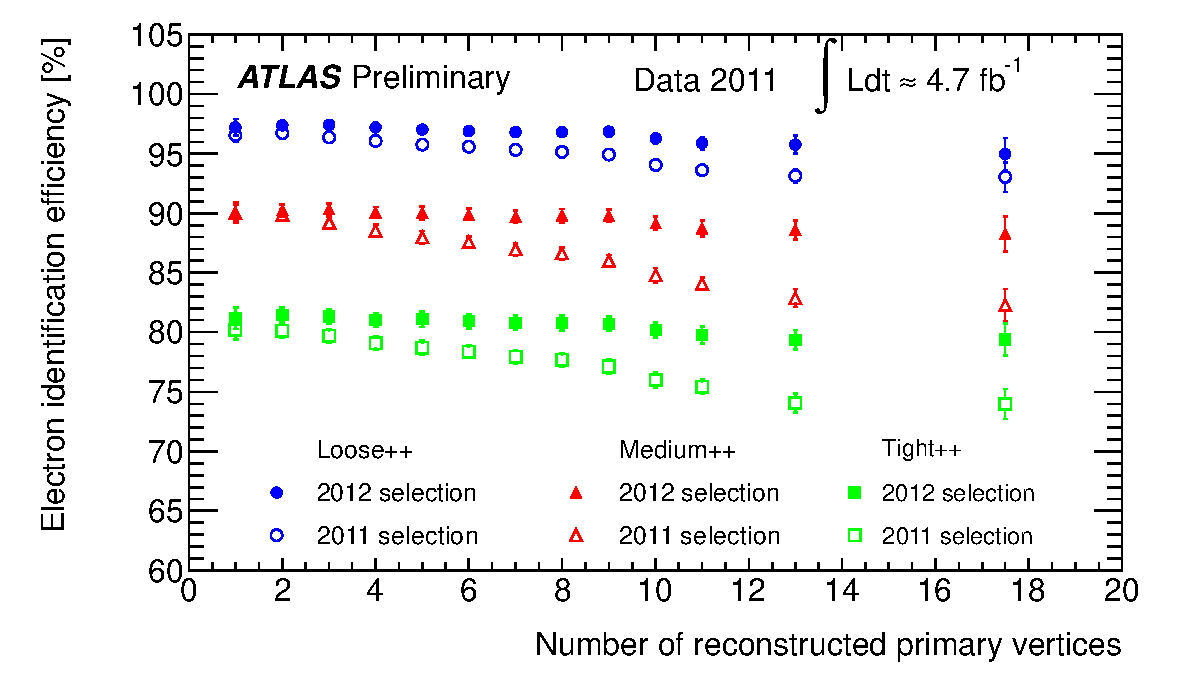
\includegraphics[width=0.80\textwidth]{figs/electron/data_effPP_vs_pvx}
\caption{Comparison of the efficiency of the 2011 and 2012 electron identification menus versus the number of primary vertices in the event.}
\label{figure:electron_2012_2011}
\end{figure}


\subsection{Electron Likelihood}

A natural step forward for the electron identification is the use of multi-variate algorithms. Multi-variate identification algorithms use many identification variables at once. Signals and backgrounds can be separated in a multi-dimensional variable space in ways that go beyond simple rectangular cuts. For the case of electron identification, it was found that using a likelihood function, trained with electron identification variables, provided clear performance gains with respect to rectangular cuts, while also providing stable and easily understandable results. The likelihood scores each electron based on how signal-like or background-like it is for each identification variable and then multiplies these individual scores together into a final score. Figure~\ref{figure:electron_lh_example} shows the example output of the likelihood for real electrons and fake electrons. The output distributions can be cut on continuously to produce a curve of possible selections rather than a single selection point. 

\begin{figure}[!t]
\centering 
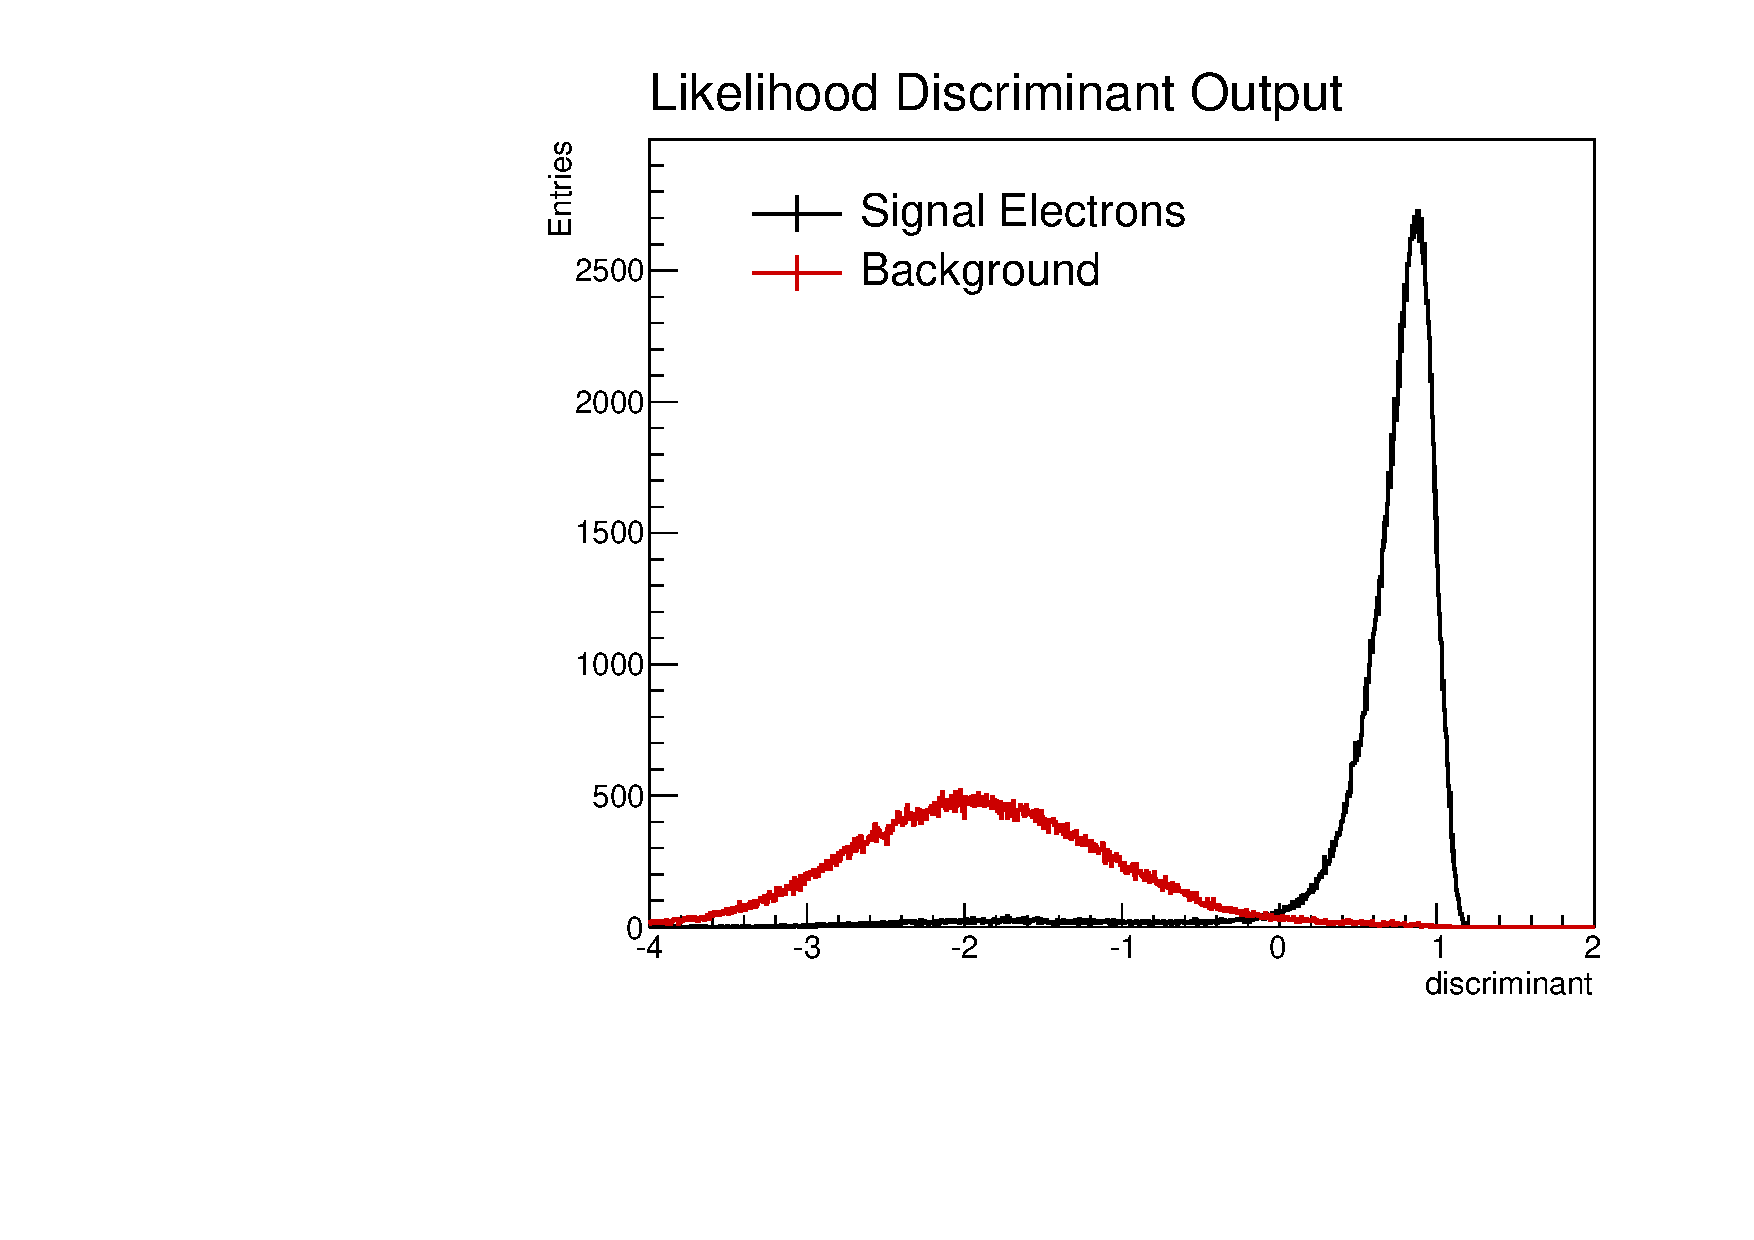
\includegraphics[width=0.40\textwidth]{figs/electron/example_lh_output}
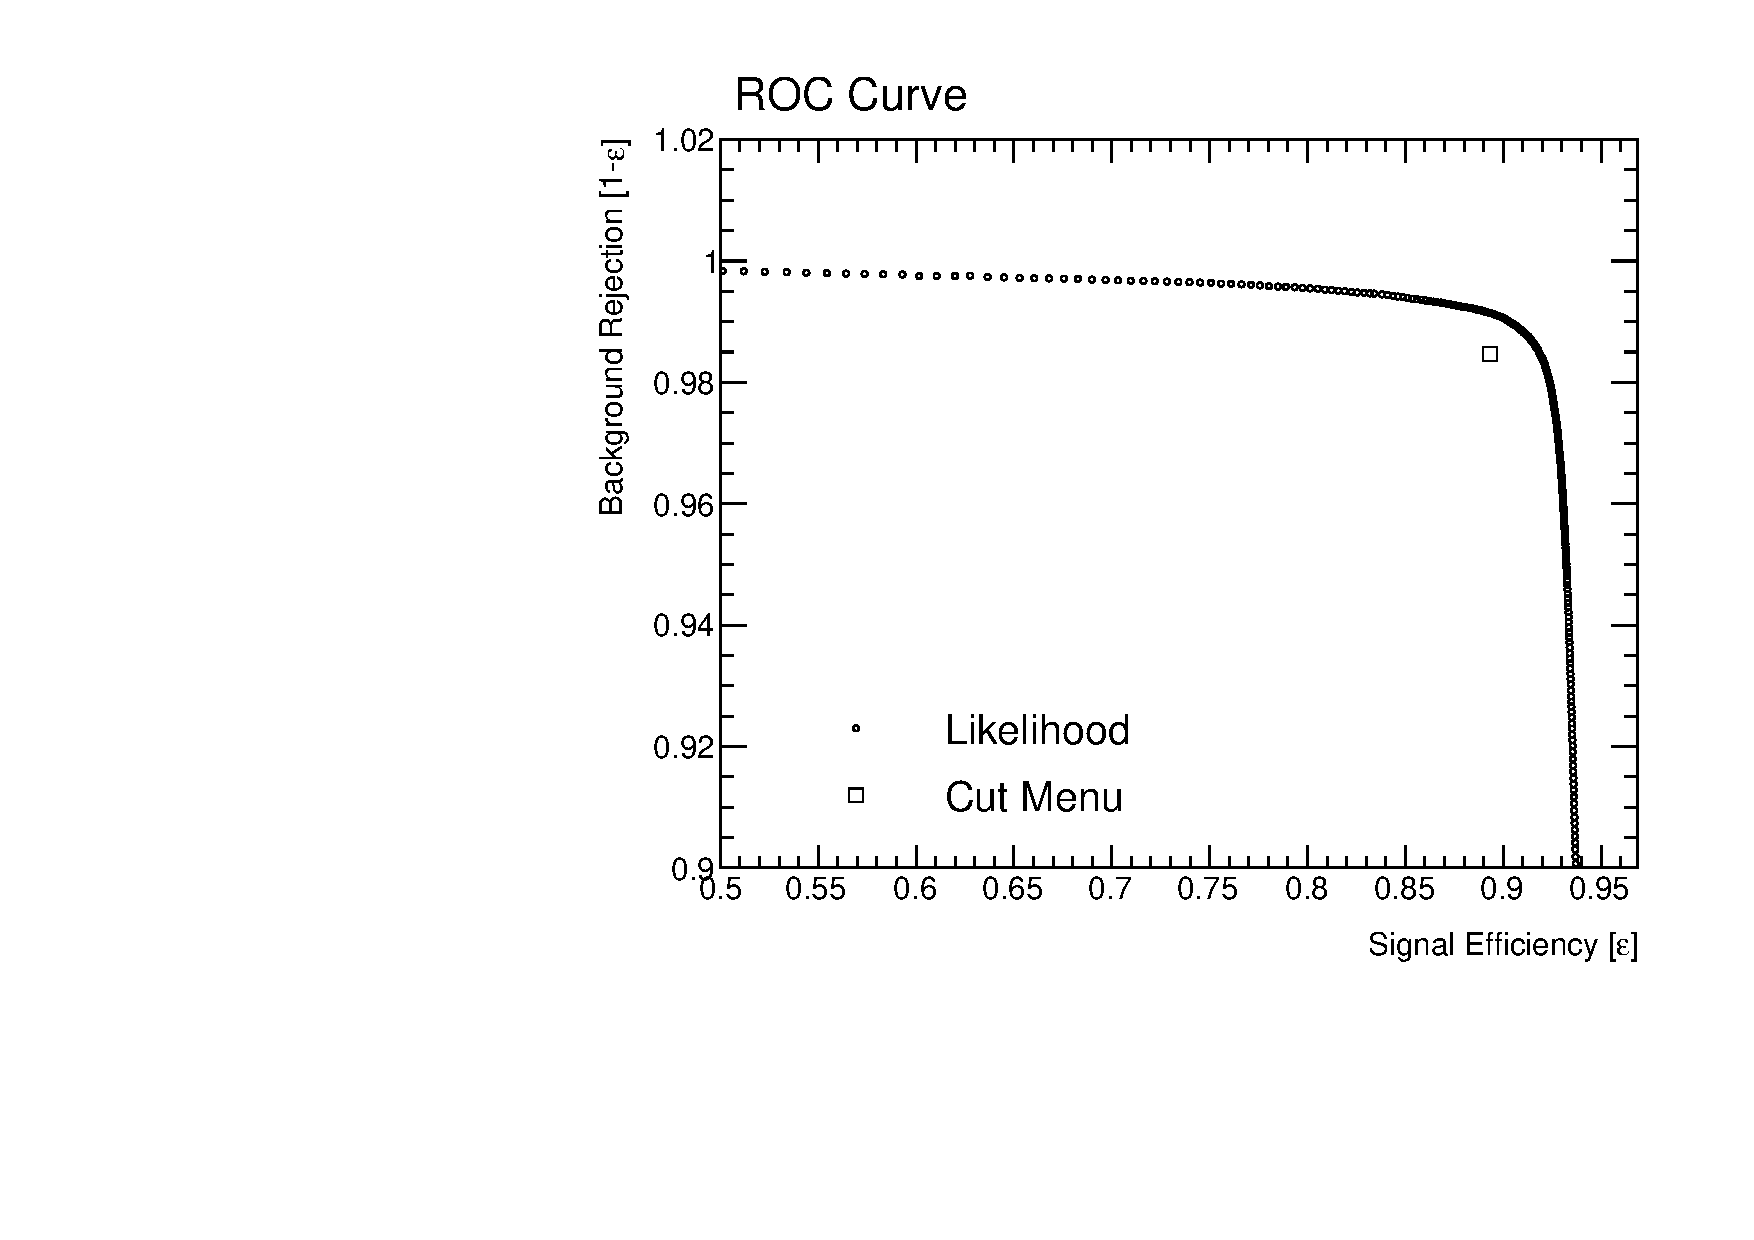
\includegraphics[width=0.40\textwidth]{figs/electron/example_roccurve}
\caption{Example electron likelihood score output for electrons and fake electrons (left). A cut can be made at any point in this distribution to define a selection operating point (right). The cut-based operating point lies within the curve of possible likelihood operating points, showing that the likelihood indeed outperforms the cuts.} 
\label{figure:electron_lh_example}
\end{figure}



There are many advantageous to a likelihood-based approach. First, variables that show significant shape differences between real and fake electrons but do not have a clear cut point can still be used in a likelihood. Second, the likelihood score takes into account the entire shape of the distribution and not simply an efficiency and fake rejection at a single cut point. Finally, the final cut on the likelihood output score can be tuned easily to achieve a desired efficiency and rejection in a way that does not overly bias selection on a single variable. 

The likelihood menu for ATLAS was developed at the end of the 2012 run to be used on advanced 2012 analyses. The menu uses similar variables to the cut-based menus but adds a few additional ones, including a measurement of the amount of energy the electron track lost as it traversed the ID. The likelihood menu makes cuts on the likelihood output score at 4 different operating points with the same binning as the cut menu but tunes the cuts based on the number of primary vertices in the event. This tuning ensures a stabile response of the identification with varying degrees of pile-up. The likelihood menu greatly outperforms the rejection of the `IsEM$++$' menu for similar efficiencies. Figure~\ref{figure:electron_cutvslh} shows a comparison of performance the cut-based and likelihood tight regime operating points. The likelihood menu, specifically the \textsc{verytight} operating point, is used in the \tth\ analysis.  

\begin{figure}[!t]
\centering 
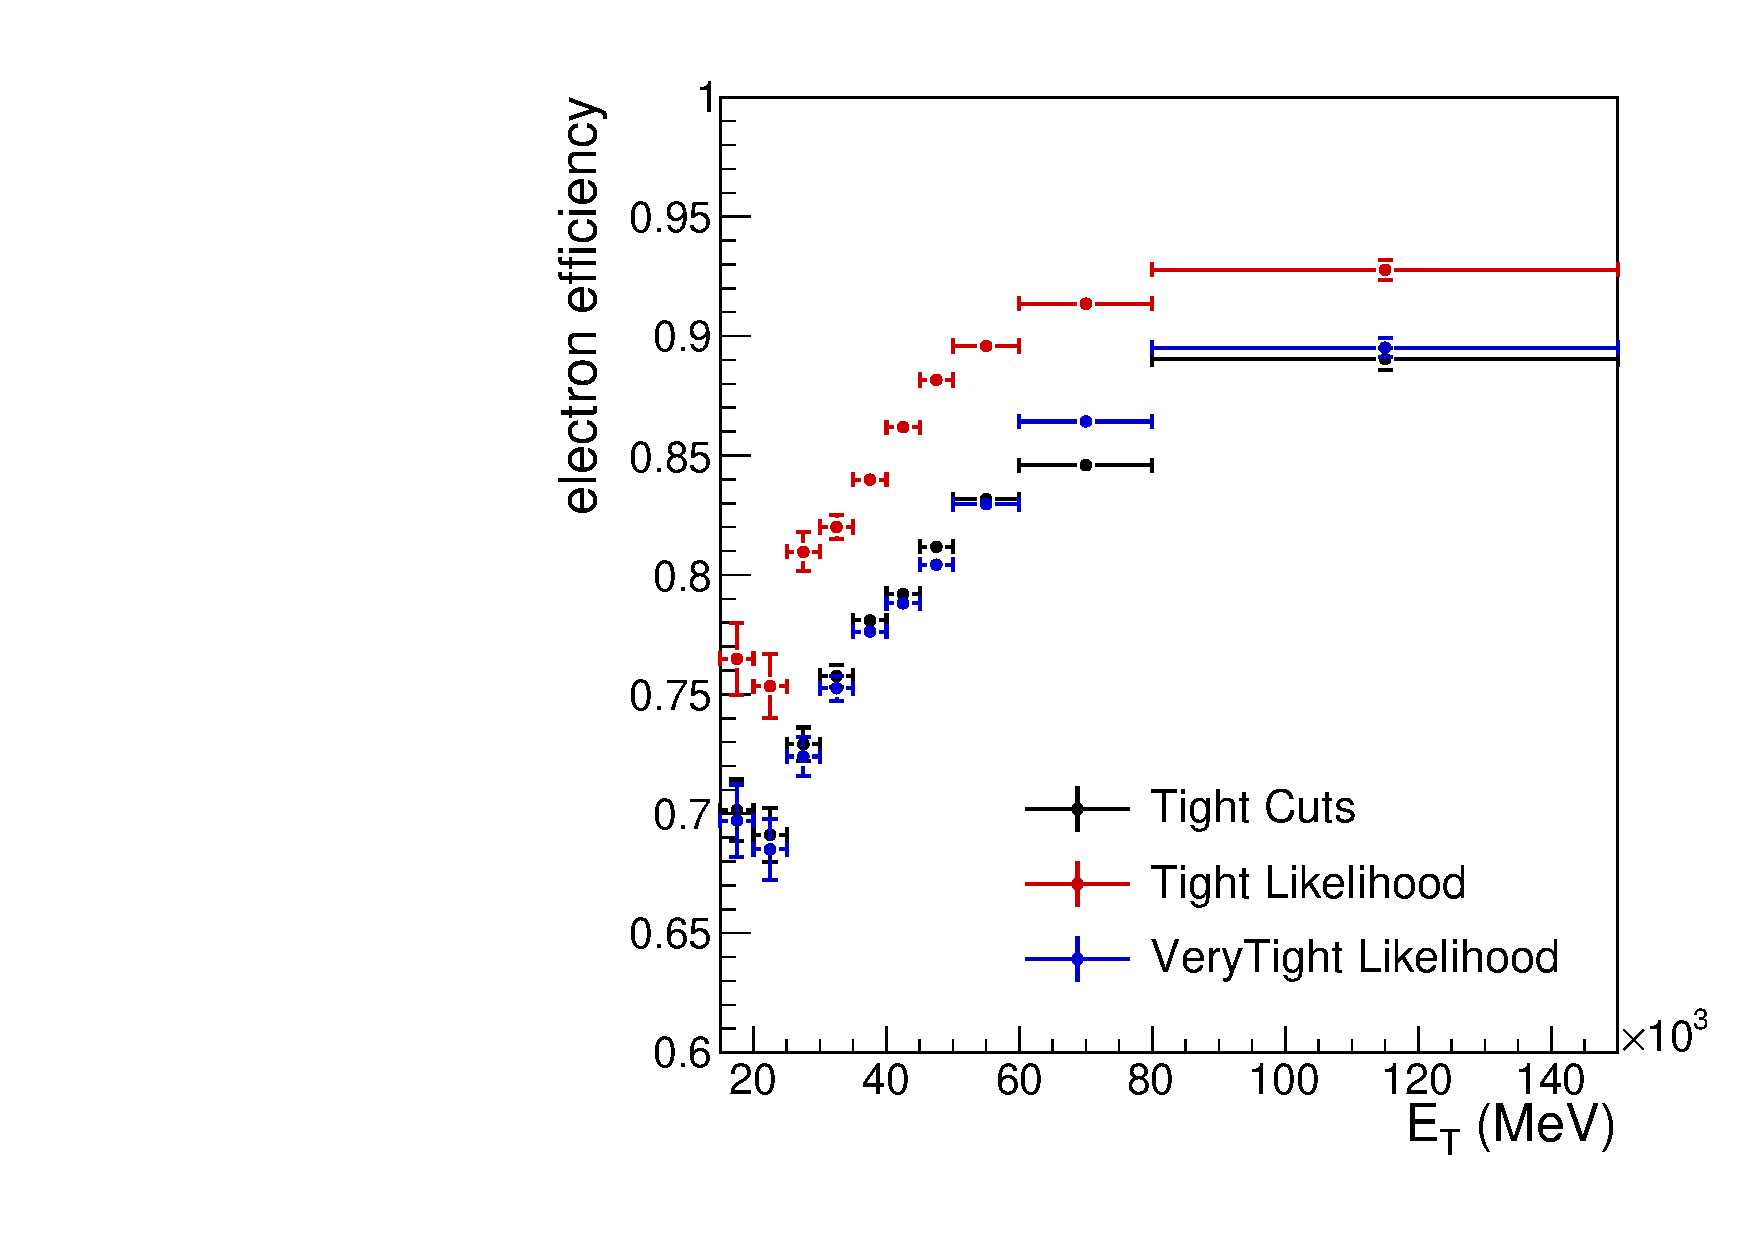
\includegraphics[width=0.40\textwidth]{figs/electron/tight_eff_et}
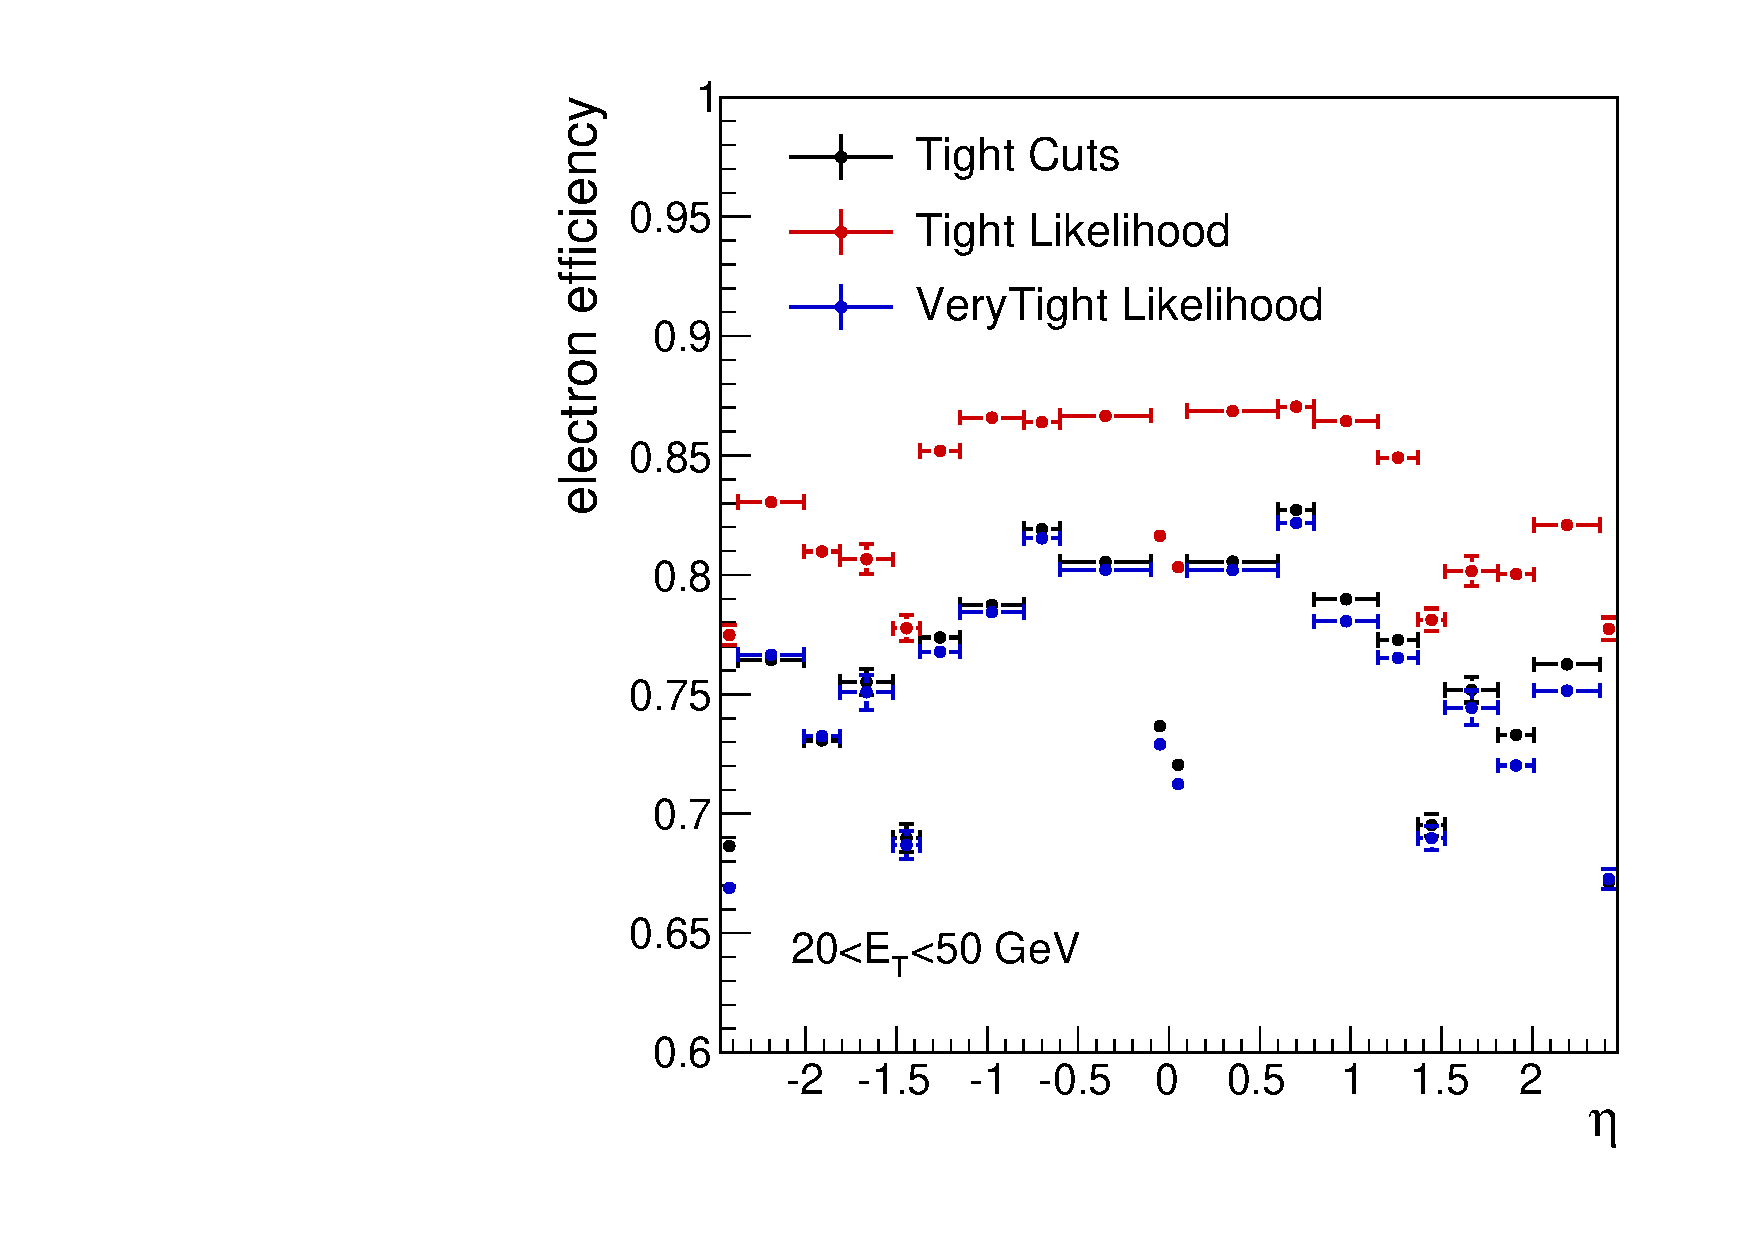
\includegraphics[width=0.40\textwidth]{figs/electron/tight_eff_eta}
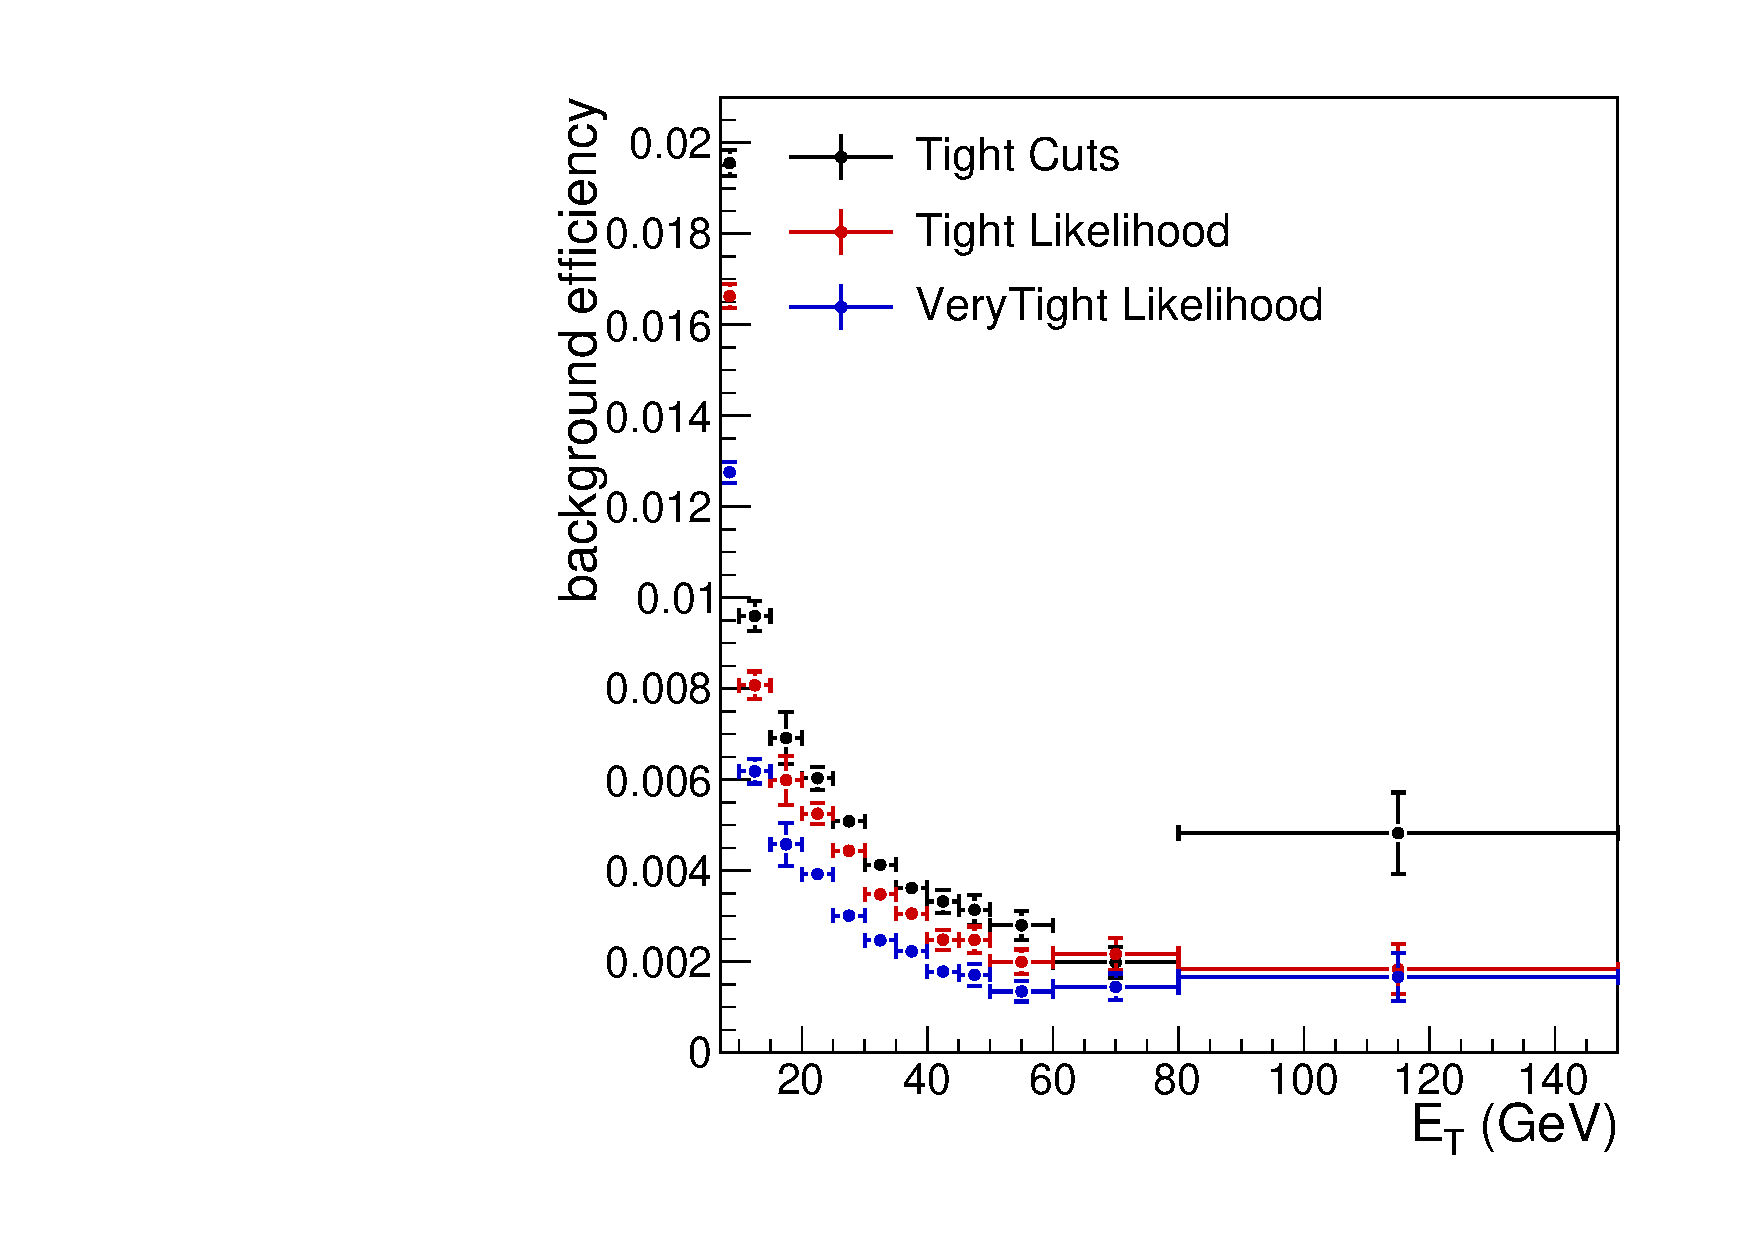
\includegraphics[width=0.40\textwidth]{figs/electron/tight_bkg_et}
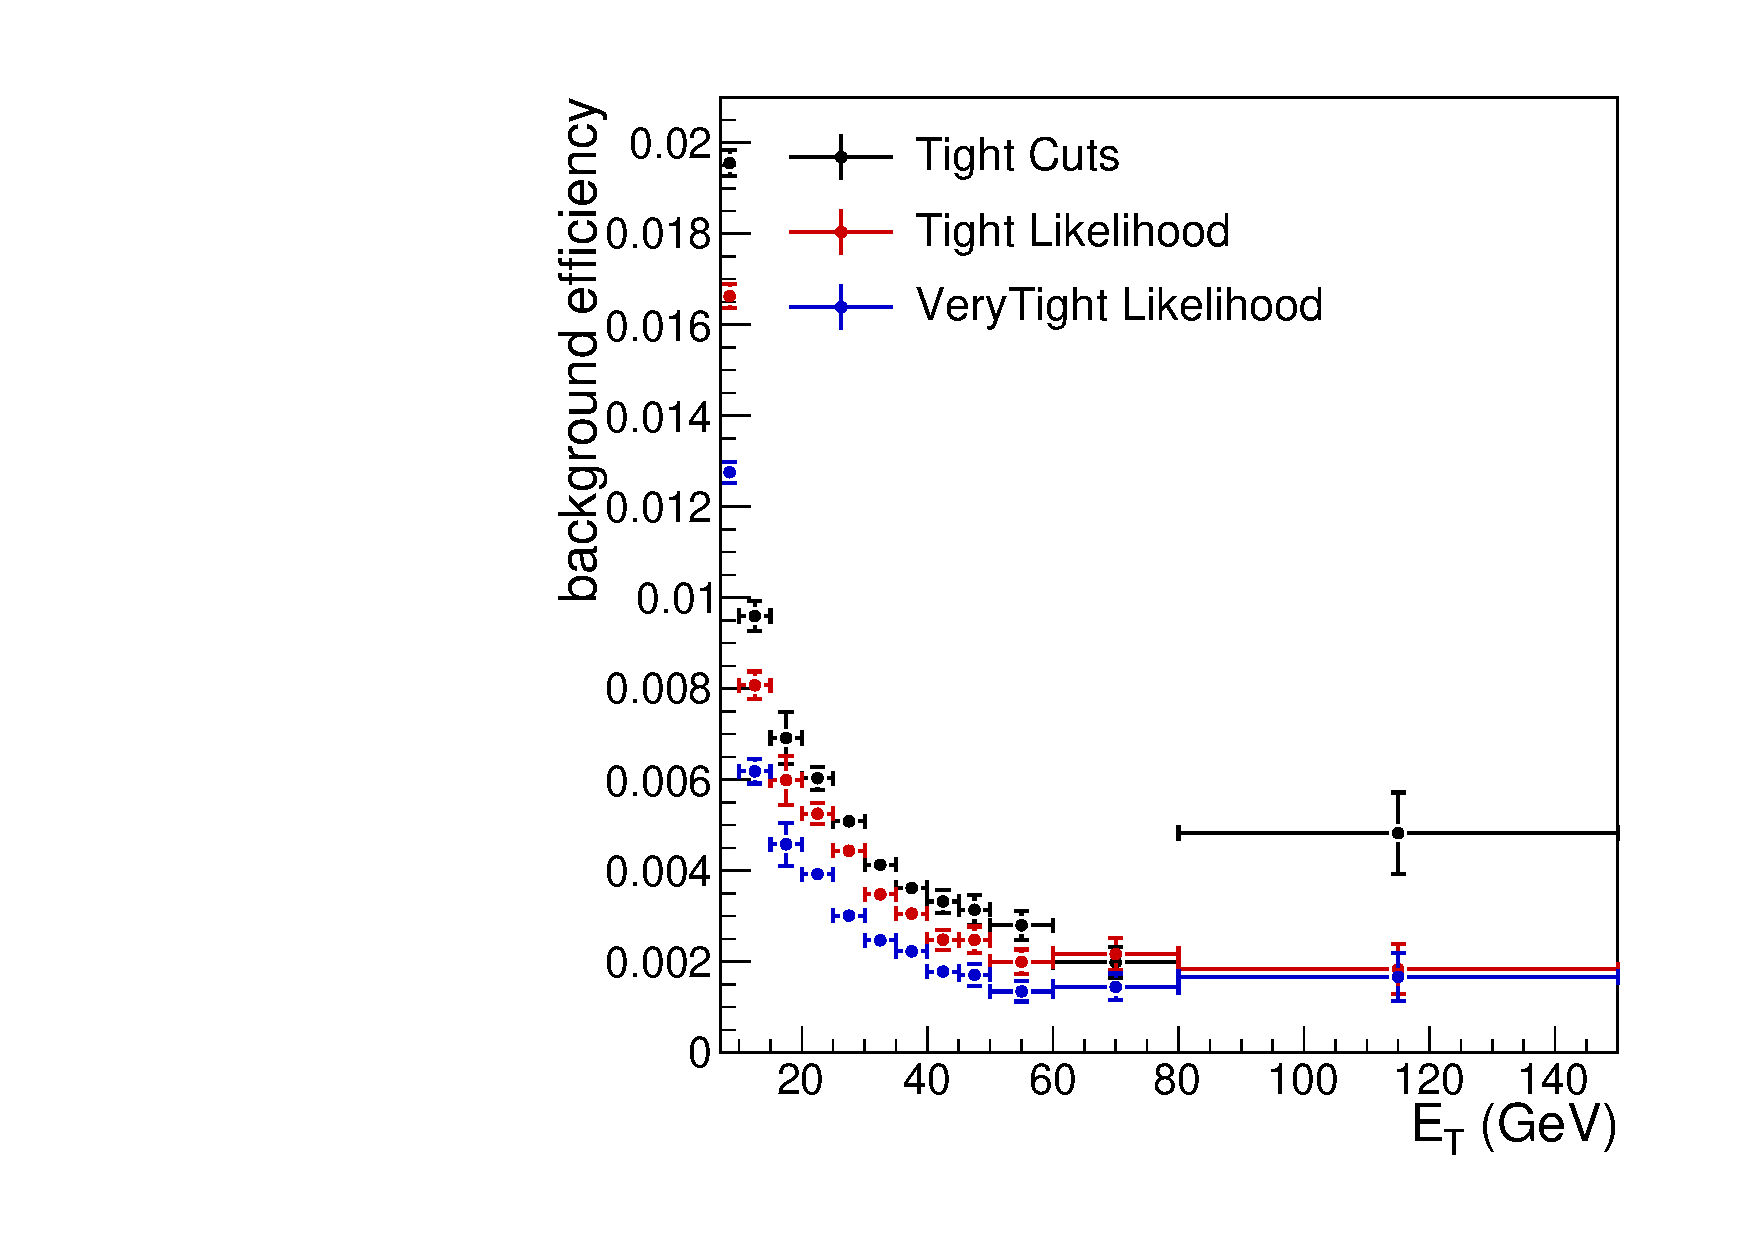
\includegraphics[width=0.40\textwidth]{figs/electron/tight_bkg_et}
\caption{Comparison of the performance of the cut-based and likelihood operating points in the tight regime. Efficiency (top) and rejection (bottom) plots are shown versus $|\eta|$ and $\et$}
\label{figure:electron_cutvslh}
\end{figure}

\section{Measurement of Electron Identification Efficiency at ATLAS}

Precise measurements of the electron identification efficiency are important pieces of many ATLAS analyses, including the \tth\ multi-leptons analysis. For analyses with low \pt\ leptons, systematic uncertainties on the electron identification efficiency can be some of the largest systematic effects. The methods used to measure the electron identification efficiency are described in depth here \cite{ATLAS-CONF-2014-032}. 

Electron identification efficiencies are measured using a method called tag-and-probe for $J/\Psi$ and $Z$ boson decays to electrons. One object from the decay is `tagged', or fully identified, while the other is left unidentified. There is reasonable confidence that the second object is an electron based on the kinematic properties of the event, specifically the di-electron invariant mass is near the $Z$ or $J/\Psi$ pole. The tag-and-probe method leaves a sample of unidentified and unbiased `probes', where the efficiency can be measured.

\begin{figure}[!t]
\centering 
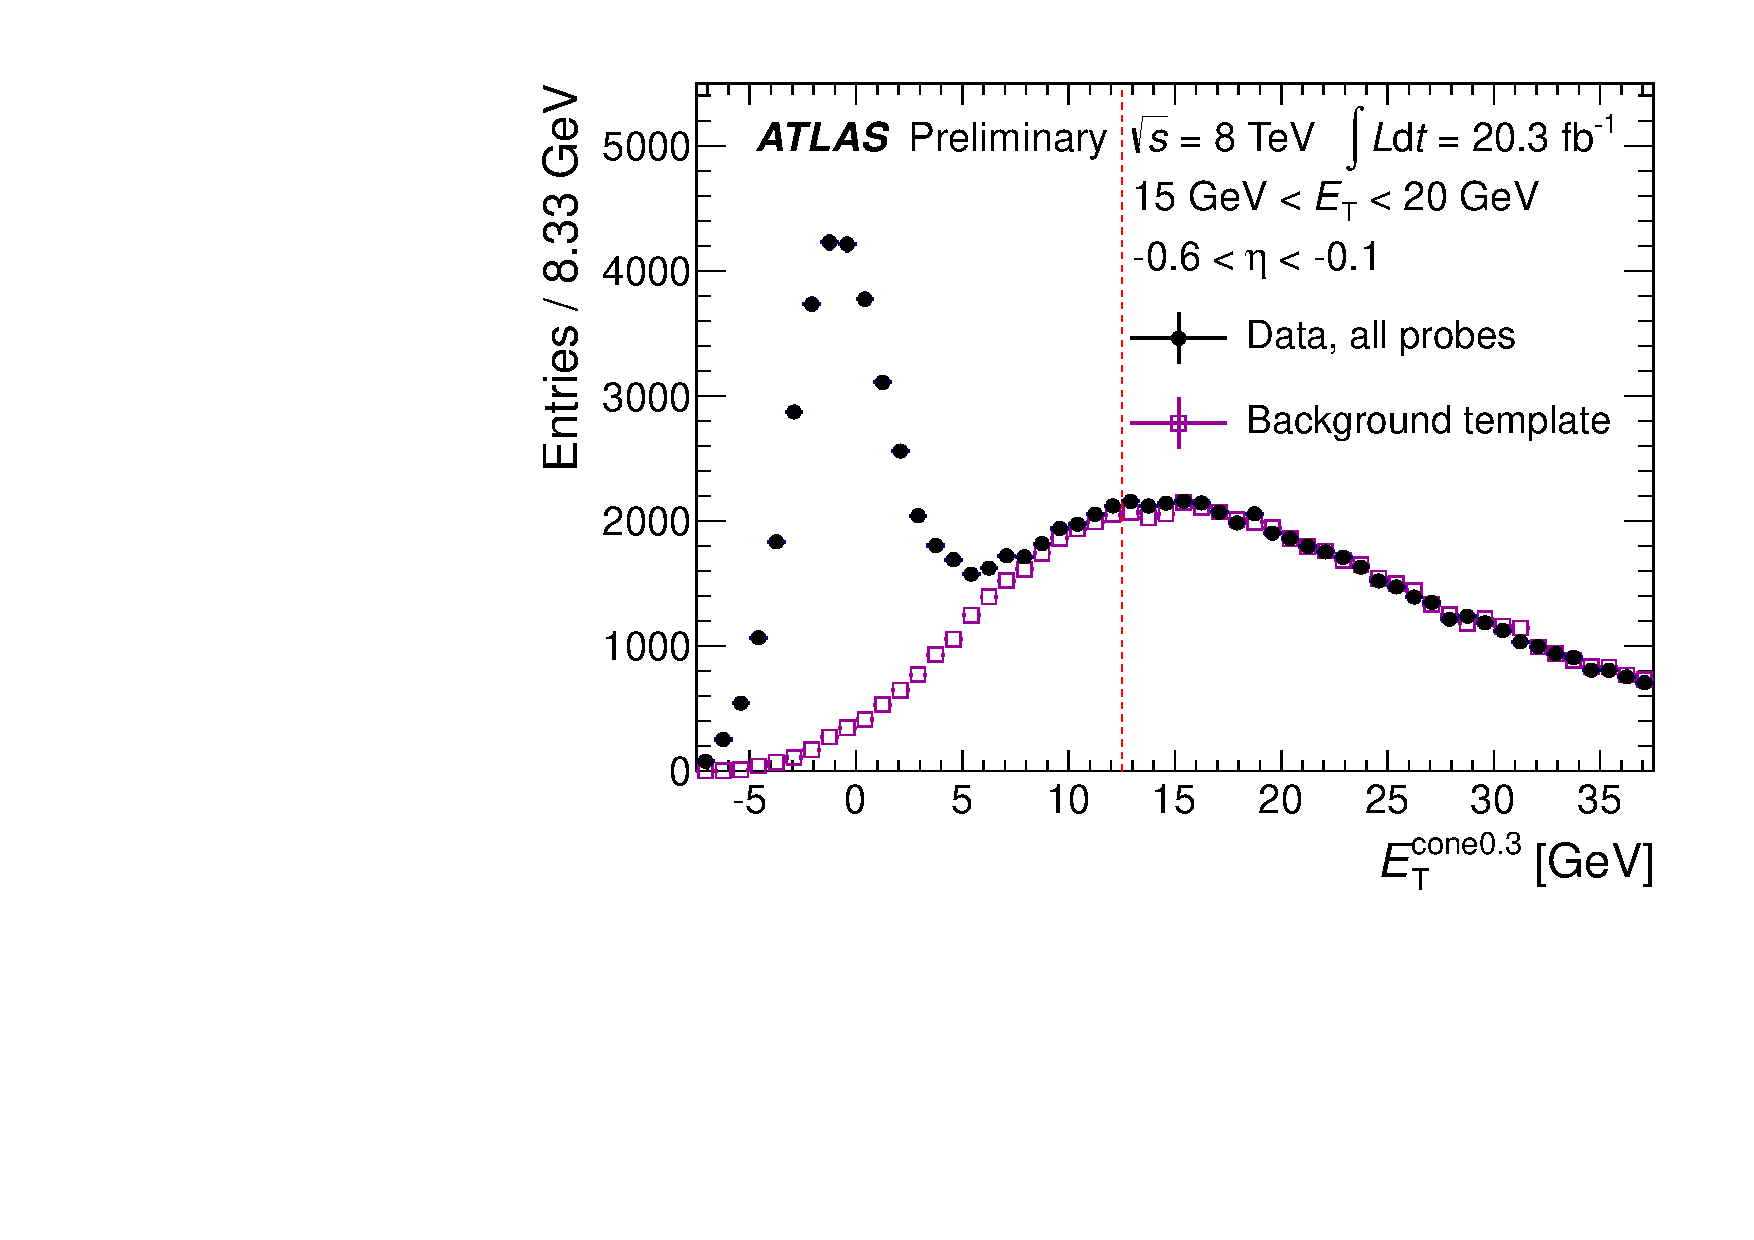
\includegraphics[width=0.40\textwidth]{figs/electron/fig_06a}
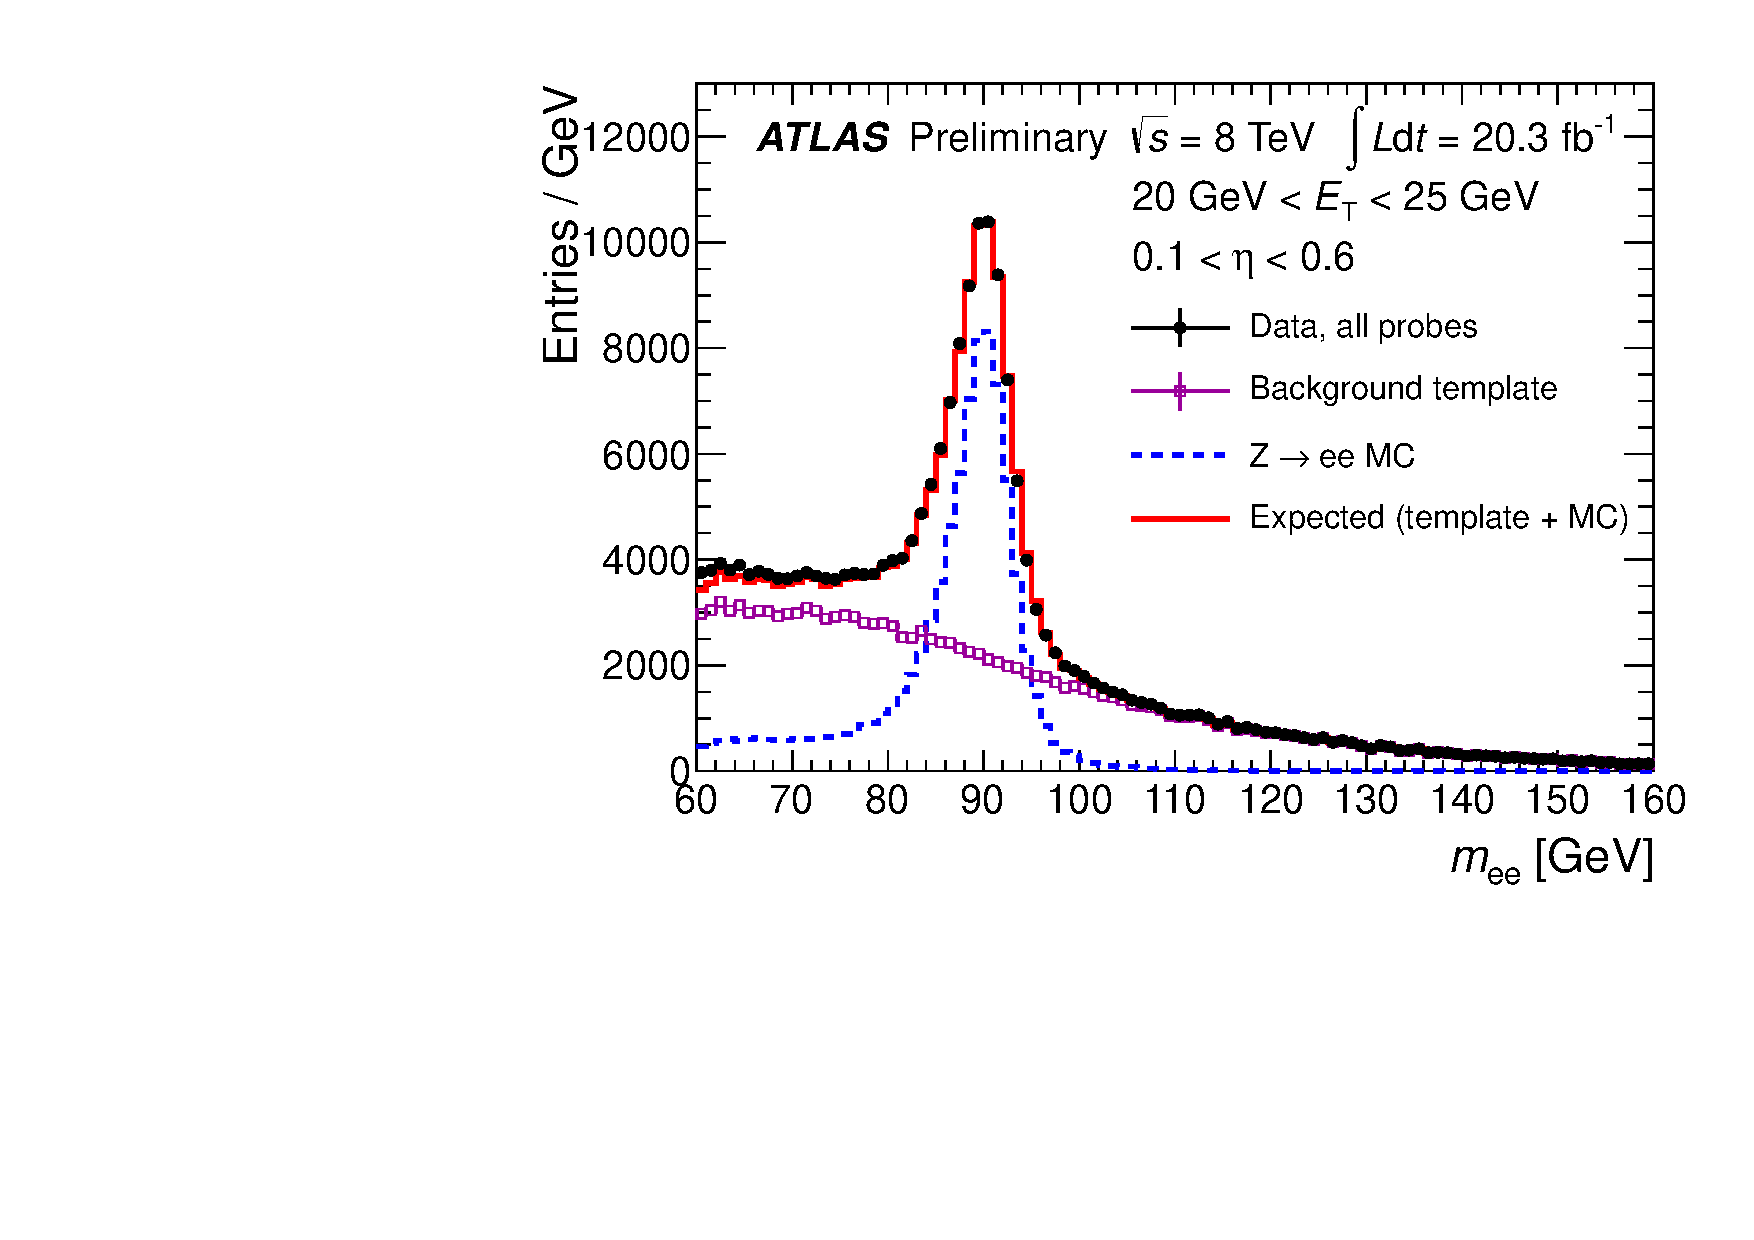
\includegraphics[width=0.40\textwidth]{figs/electron/fig_04a}
\caption{Example bins where the electron probe distribution from $Z$ tag-and-probe is fit by an isolation template (left) invariant mass template (right) to subtract backgrounds.} 
\label{figure:electron_probe}
\end{figure}


As opposed to muons, contamination from fake electron make the tag-and-probe method difficult. Backgrounds from fake electrons are subtracted using fits to the $Z$ and $J/\Psi$ invariant mass distributions. For $Z$ electrons, fits to the electron isolation distribution are also used. The final efficiencies reported are the result of statistical fit among all methods. The uncertainties are at low momenta are around $\sim$ 5\% and are dominated by systematics effects from large background subtractions. They are less than 1\% at high momenta and dominated by tag-and-probe selection effects. The efficiency can be seen in Figure~\ref{figure:electron_eff}. 

\begin{figure}[!t]
\centering 
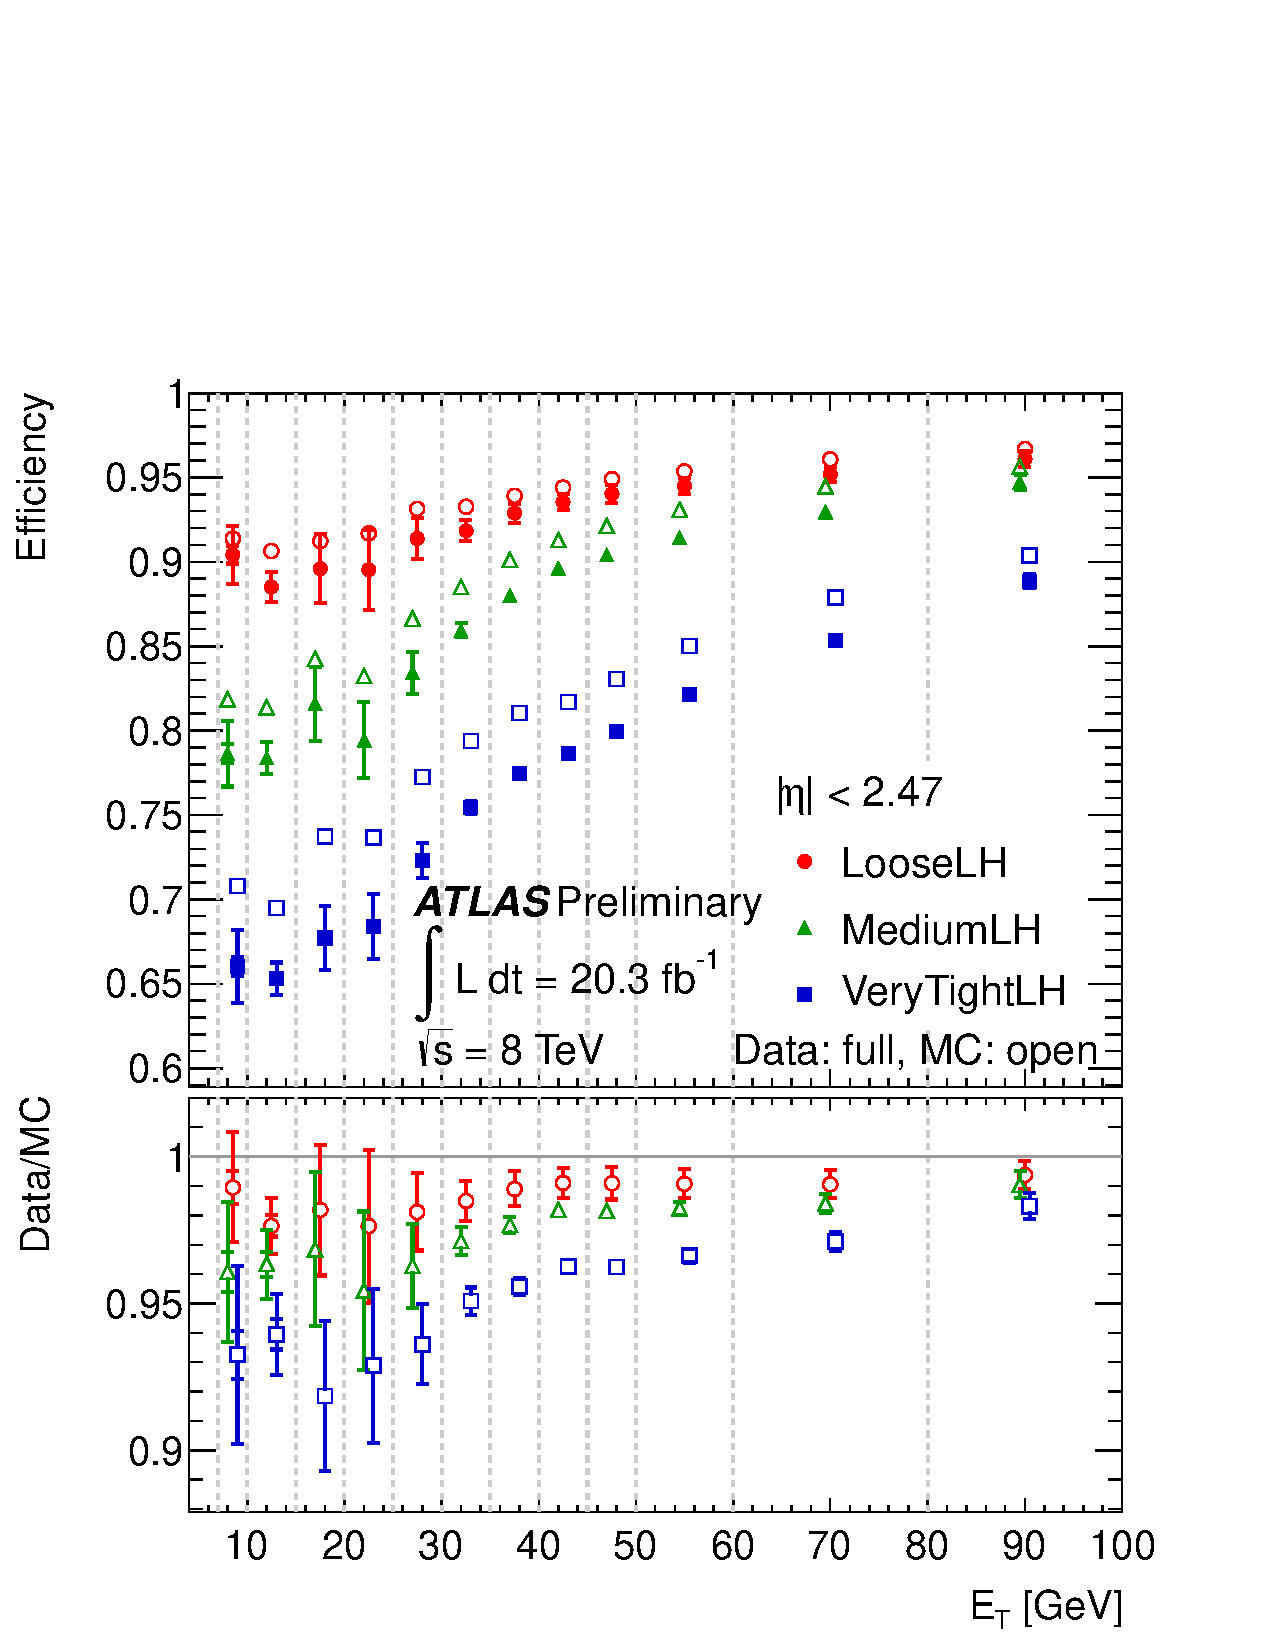
\includegraphics[width=0.60\textwidth]{figs/systematics/fig_22a}
\caption{Electron identification efficiency calculated in data and MC versus electron \pt.} 
\label{figure:electron_eff}
\end{figure}

The development of low \pt\ electron scale-factors was an integral piece in extending the sensitivity of Higgs searches in the $WW$ and $ZZ$ decays modes. Early efforts in 2012 to provide consistent, well-measured efficiencies in this region were complicated by large disagreements in the efficiencies obtained from the three different estimation methods: $Z$ tag-and-probe with isolation background subtraction, $Z$ tag-and-probe with invariant mass background subtraction, and $J/Psi$ tag-and-probe. This was especially true for electrons with \pt\ of 10-20 GeV. The energy scale of $Z$ and $J/\Psi$ decays disfavor electrons of this momentum, and backgrounds are high, revealing problems disguised in higher purity regions. The background subtraction methods were studied in depth to assess possible biases, and a new lower statistics but high purity tag-and-probe method using radiative $Z\rightarrow ee\gamma$ decays was developed. The result of these studies was the development of new background subtraction templates for the isolation and invariant mass subtraction and an appropriate uncertainty to cover the systematic effects from the biases of these subtractions.



